% SufficiencyBench -- ACM TOIS submission (single-blind)
\documentclass[acmsmall,screen,review]{acmart}
\acmJournal{TOIS}
\acmYear{2026}
\usepackage{enumitem}
\newcommand{\bench}{SufficiencyBench}
\newcommand{\sprobe}{SufficiencyProbe}
\graphicspath{{./}}
\title[Will the Retrieved Context Suffice?]{Will the Retrieved Context Suffice? Confound-Controlled Evaluation of Sufficiency Predictors for Retrieval-Augmented Generation}
\author{Guillermo Llopis-Garc\'ia}
\orcid{0009-0001-9985-6516}
\affiliation{\institution{Instituto de Neurociencia Avanzada de Barcelona (INAB)}\city{Barcelona}\country{Spain}}
\affiliation{\institution{Department of Computer Technology, University of Alicante}\city{San Vicente del Raspeig}\country{Spain}}
\email{g.llopis@inablab.org}
\author{Daniel Ruiz-Fern\'andez}
\orcid{0000-0002-8919-8863}
\affiliation{\institution{Department of Computer Technology, University of Alicante}\city{San Vicente del Raspeig}\country{Spain}}
\email{druiz@ua.es}
\author{David del Rosario Gilabert}
\orcid{0009-0000-4271-8799}
\authornote{Corresponding author.}
\affiliation{\institution{Instituto de Neurociencia Avanzada de Barcelona (INAB)}\city{Barcelona}\country{Spain}}
\email{d.delrosario@inablab.org}
\renewcommand{\shortauthors}{Llopis-Garc\'ia et al.}

\begin{document}
\begin{abstract}
A retrieval-augmented generation (RAG) system should answer only when the retrieved context suffices. Deciding this is a generation-stage performance-prediction problem, the counterpart of query performance prediction, and common predictors read the model's output. On natural retrieval data two confounds inflate their scores: answer-bearing passages differ in length, and a model that knows the answer is confident regardless of the context. \bench{} is a 5,370-example benchmark whose insufficient contexts are minimally edited, length-matched copies of the sufficient ones, with labels stratified by closed-book knowledge and validated by annotation. Eighteen predictors are compared on three open-weight models, fewer on three more and on two frontier API models. No zero-shot output-based predictor, logit-based included, reaches 0.83 AUROC on any model; a linear probe on intermediate hidden states reaches 0.90--0.95. The gap survives scale, model family, chain-of-thought prompting and a readout trained on the output scores, and a text-only encoder trained on the same labels matches the probe: the ceiling limits what the output exposes, not the task. Since the edit is itself a cue for trained readers, the ordering is confirmed on unedited retrieved contexts against query performance predictors; it shrinks under source shift and long contexts and yields three deployment tiers.
\end{abstract}

\begin{CCSXML}
<ccs2012>
<concept>
<concept_id>10002951.10003317.10003347.10003348</concept_id>
<concept_desc>Information systems~Question answering</concept_desc>
<concept_significance>500</concept_significance>
</concept>
<concept>
<concept_id>10002951.10003317.10003359.10003361</concept_id>
<concept_desc>Information systems~Retrieval effectiveness</concept_desc>
<concept_significance>300</concept_significance>
</concept>
<concept>
<concept_id>10010147.10010178.10010179</concept_id>
<concept_desc>Computing methodologies~Natural language processing</concept_desc>
<concept_significance>300</concept_significance>
</concept>
</ccs2012>
\end{CCSXML}

\ccsdesc[500]{Information systems~Question answering}
\ccsdesc[300]{Information systems~Retrieval effectiveness}
\ccsdesc[300]{Computing methodologies~Natural language processing}

\keywords{retrieval-augmented generation, context sufficiency, query performance prediction, selective answering, abstention, hidden-state probing, evaluation methodology}

\maketitle

\section{Introduction}
\label{sec:introduction}

Large language models (LLMs) deployed with retrieval-augmented generation (RAG) \citep{lewis2020rag} condition their responses on passages retrieved at inference time. Retrieval does not always succeed: the ranked list may miss the evidence, split it across passages, or return text that is topically related but does not answer the question, and in all of these cases the generator tends to answer anyway \citep{joren2025sufficient,cuconasu2024power}. A RAG system therefore needs a score, computed before or during generation, that tells it whether the retrieved context \emph{suffices} for the question, so that it can abstain, retrieve again or hand the question to a person. We call this \emph{context sufficiency prediction}. It is the generation-stage counterpart of query performance prediction (QPP), which estimates retrieval effectiveness without relevance judgments \citep{cronentownsend2002predicting,shtok2012predicting,carmel2010estimating}, and it has recently been taken up from the IR side as the prediction of retrieval utility or RAG benefit \citep{tian2026predicting,sinha2026adaptive,dado2026benefit}. Where QPP asks whether the ranking is good, sufficiency prediction asks whether what was retrieved lets this model answer this question, which is a utility judgment rather than a relevance judgment \citep{zhang2024utility}. The label is a property of the question and the retrieved context, not of the generator; what depends on the generator is how much of that label each predictor recovers, and from where.

Most predictors in use read the model's output: verbalized confidence (VC) \citep{xiong2024llms,kadavath2022language}, semantic entropy \citep{farquhar2024semantic}, attention-based decompositions of the answer \citep{sun2025redeep}, and the uncertainty signals that adaptive-retrieval systems use to decide whether to retrieve at all \citep{jiang2023active,su2024dragin,moskvoretskii2025adaptive}. They report an area under the receiver operating characteristic curve (AUROC) above 0.78 on their respective benchmarks. A second line reads the model's hidden states instead and finds that properties of its belief are linearly decodable \citep{azaria2023internal,marks2024geometry}, including, for RAG, whether another retrieval round is needed \citep{baek2025probingrad,niu2026uarag,yao2025seakr,liu2025ctrla} and how much retrieval will help \citep{dado2026benefit}. What neither line establishes is how the two relate. Output-based and hidden-state predictors have been evaluated on different data, under different confounds and with different amounts of supervision, so it is not known whether the output-based scores are approaching a limit set by what the output exposes, or whether the gap to a trained probe is an artefact of training, of evaluation data, or of nothing at all.

The question cannot be settled on natural retrieval data alone, because two confounds inflate output-based scores there. In the HotpotQA distractor setting the passages that support the answer are shorter than the distractors, and passage length alone separates supporting from distractor paragraphs at 0.65 AUROC, so a predictor can score well without reading the content (Section~\ref{sec:validity}). And when a model has memorised the answer from pretraining, its output is confident whether or not the retrieved context contributed \citep{mallen2023trust,ren2025investigating}. Prior evaluations of sufficiency and abstention \citep{joren2025sufficient,kirichenko2025abstentionbench,peng2025unanswerability} control for neither at once. This is the RAG instance of a familiar evaluation problem: a test collection whose labels co-vary with a surface variable rewards predictors that read the surface variable.

We therefore build \bench{}, a benchmark whose sufficient and insufficient contexts differ only in the answer-bearing sentence and whose labels are stratified by each model's own prior knowledge, and use it to compare 18 predictors on three 7B--8B open-weight LLMs, the probes and output-based predictors on three more open-weight models, and the output-based predictors on two frontier API models, organised by where each method reads from the network: the generated output, the attention pattern, or the residual stream. Our central claim is that the output-based detectors share a ceiling that is an \emph{access limit}: whatever the generated tokens expose of the sufficiency signal is less than the residual stream carries. Three results support the claim. No zero-shot output-based method, including a logit readout, reaches 0.83 overall AUROC on any of the eight models, and the gap to a linear probe on intermediate hidden states (0.90--0.95) does not close with scale, model family, or chain-of-thought prompting. A readout \emph{trained} on the output-based scores, under the same cross-validation as the probes, stays within about 0.03 of each model's zero-shot verbalized confidence, so supervision does not explain the gap. And on the three models where all three access points were measured, detection improves in the order outputs, attention, residual stream, with the classifier type held fixed, a trained linear classifier, across the two internal access points; a layer sweep is consistent with this ordering, since the same probe loses 0.06 to 0.08 AUROC between its selected layer and the final layer. We then test the ordering where it has to hold to matter, on contexts produced by a real retriever: BM25 over the pooled HotpotQA paragraphs, top-$k$ passages concatenated, sufficiency labelled by whether every gold-support paragraph was retrieved, and retriever-score predictors from QPP as baselines (Section~\ref{sec:retrieved}). Finally we bound the claim: the probe's advantage shrinks on a held-out source dataset, and when the passage is buried in long contexts the probe trained on short passages loses most of its margin while only a probe retrained at that length keeps one, up to 32,000 tokens, so the result is specific to retrieved contexts of a few hundred tokens.

The contributions of this paper are the following.
\begin{enumerate}[leftmargin=*,topsep=2pt,itemsep=1pt]
\item An evaluation methodology for context sufficiency prediction and its instance, \bench{}: a 5,370-example benchmark that removes the passage-length and parametric-knowledge confounds by construction, with labels validated by human annotation, surface-feature and editing-cue controls and label-noise robustness, released with the evaluation pipeline and the code that trains and scores the probes.
\item An 18-predictor, eight-model comparison organised by access point, showing that no zero-shot output-based predictor approaches a linear probe on intermediate hidden states, that training a readout on the output-based scores does not close the gap, and that prediction improves from output to attention to residual stream on the three models where all three were measured. We read this as an access limit on output-based prediction.
\item The scope of the result: its persistence on BM25-retrieved contexts against QPP baselines, the probe's margin under source-dataset shift, its loss at 4,000 to 100,000 tokens, and three deployment tiers, verbalized confidence, a single-forward-pass probe, and a 395M standalone encoder that needs no LLM, with their latency and accuracy trade-offs.
\end{enumerate}

\section{Related Work}
\label{sec:related}

\paragraph{Predicting retrieval and generation performance.}
Query performance prediction estimates how well a retrieval system served a query without relevance judgments, from pre-retrieval statistics of the query \citep{zhou2007query,hauff2008survey} or post-retrieval statistics of the ranked list such as clarity \citep{cronentownsend2002predicting}, query drift \citep{shtok2012predicting} and their supervised and conversational successors \citep{carmel2010estimating,arabzadeh2021bertqpp,datta2022deepqpp,datta2022pointwise,meng2023qppconv,faggioli2026introduction}, with its own evaluation methodology \citep{faggioli2022smare}, and it has been extended to LLM-generated relevance judgments \citep{meng2025query} and query variants \citep{tian2026raqgqpp} and examined for its failure modes under selective query processing \citep{chifu2026uncovering}. With RAG, the quantity to predict moved downstream. \citet{sinha2026adaptive} predict retrieval effectiveness from post-retrieval features and use it to adapt retrieval depth; \citet{tian2026predicting} predict retrieval utility and answer quality; \citet{salemi2024evaluating} evaluate retrieval by the downstream answer it produces, and RAG evaluation frameworks score context relevance and answer faithfulness with LLM judges \citep{es2024ragas,saadfalcon2024ares}; and \citet{dado2026benefit} predict the benefit of retrieving over answering closed-book, comparing pre-retrieval, post-retrieval and post-generation predictors with a probe that adapts the LLM's final hidden states, and find that the probe narrows but does not close the gap to a supervised post-generation predictor. Adaptive-retrieval systems make the same decision online, from the model's own uncertainty \citep{jiang2023active,su2024dragin,wang2023skr,moskvoretskii2025adaptive}, from question complexity \citep{jeong2024adaptive}, from a retrieval evaluator that grades each passage \citep{yan2024corrective}, or from the knowledge the model already has \citep{mallen2023trust,ren2025investigating}. Our question is narrower and prior to all of these: given the context a retriever returned, how well can a predictor tell whether it suffices, and does the answer depend on where the predictor reads? The closest work, \citet{dado2026benefit}, predicts a continuous gain on natural retrieval data with a single, adapted access point; we hold the predictor fixed as a linear readout, vary the access point, and remove the confounds that natural data carry. \citet{zhang2024utility} show that LLMs judge utility differently from relevance; sufficiency is a utility judgment about the retrieved set, and \citet{cuconasu2024power} show that the composition of that set, including irrelevant passages, changes what the generator produces, which is why we evaluate on retrieved contexts as well as on edited ones (Section~\ref{sec:retrieved}).

\paragraph{Sufficiency and abstention in RAG.}
\citet{joren2025sufficient} introduced an autorater for whether a retrieved context suffices and showed that models answer rather than abstain even when it does not; AbstentionBench \citep{kirichenko2025abstentionbench} and UAEval4RAG \citep{peng2025unanswerability} measure the same failure on unanswerable questions, and selective question answering studies the resulting risk--coverage trade-off \citep{kamath2020selective}. Self-RAG trains the model to emit reflection tokens that decide whether to retrieve and whether a passage supports the answer \citep{asai2024selfrag}, and Probing-RAG and UA-RAG read hidden states to decide whether another retrieval round is needed \citep{baek2025probingrad,niu2026uarag}; on the IR side, \citet{lajewska2024unanswerable} detect unanswerable questions in information-seeking conversations. A related line studies what happens when the retrieved evidence and the model's parametric memory disagree \citep{neeman2023disentqa,li2024conflictbank,zhao2025parametric}, or when the context is irrelevant \citep{shi2023distracted,yoran2024making}, the situations our parametric-knowledge stratification and paired construction isolate. All of these works evaluate on natural retrieval data, in which sufficiency co-varies with passage length and with what the model already knows. None controls both confounds at once, and none compares output-based and hidden-state predictors for context sufficiency on confound-controlled data.

\paragraph{Uncertainty estimation over model outputs.}
Verbalized confidence asks the model to rate its own certainty \citep{xiong2024llms}. Semantic entropy clusters sampled continuations by meaning and scores their dispersion \citep{farquhar2024semantic}, and a family of refinements reweights or restructures the clusters. Prompting the model to reason before answering is often expected to improve these scores, although the stated reasoning need not reflect the computation that produced the answer \citep{turpin2023unfaithful}. All of these methods read the output only. Whether their incremental gains are approaching a limit set by that access point is the question taken up here.

\paragraph{Detectors that read internal state.}
Latent truth directions can be found in the residual stream without supervision \citep{burns2023discovering}, a classifier on hidden states detects when the model is producing a falsehood \citep{azaria2023internal}, and truth values of factual statements form a stable linear direction across models \citep{marks2024geometry}, in line with the linear representation hypothesis \citep{park2024linear}. Probing classifiers come with known caveats about what a high probe accuracy does and does not show \citep{belinkov2022probing}, which is why we pair the probes with a steering experiment (Appendix~\ref{sec:steering_app}), and \citet{magata2026answeronly} show that for hallucination probes scored under teacher forcing, much of the separability can come from the answer tokens alone. For hallucination detection specifically, INSIDE scores the covariance of sampled hidden states \citep{chen2024inside}, the ICR Probe tracks hidden-state dynamics across layers \citep{zhang2025icrprobe}, and activations of an open-weight proxy model have been used to audit a closed one \citep{singh2026proxyanalyzer}. Attention has been read directly: the Lookback Lens classifies the share of attention that generated tokens pay to the context \citep{chuang2024lookback} and ReDeEP decomposes attention into contextual and parametric contributions \citep{sun2025redeep}. Where these detectors have been compared with hidden-state classifiers, as in \citet{chuang2024lookback}, it was on hallucination data with the confounds above uncontrolled, so the access points have not been compared on equal terms for context sufficiency. In IR, \citet{liu2026how} trace with activation patching how an LLM arrives at a relevance judgment, finding that query and document information is assembled in early and middle layers before a few late attention heads produce the verdict; our layer sweep (Appendix~\ref{sec:layers}) is the sufficiency counterpart of that picture. We extend the linear-probe result to context sufficiency, a relational property of the query and the context together, and compare output, attention and residual-stream readouts on the same confound-controlled data.

\paragraph{Confound control in evaluation.}
Benchmark scores overestimate capability when the evaluation data contain uncontrolled surface correlates: in natural language inference, hypothesis-only classifiers exploit annotation artefacts \citep{gururangan2018annotation}, models fall back on heuristics such as lexical overlap \citep{mccoy2019right}, and adversarial filtering was required before commonsense reasoning scores became reliable \citep{sakaguchi2020winogrande}. The two confounds above are the RAG instances of this pattern. \bench{} applies the standard remedies, matching on the surface variables and stratifying on the nuisance variable, and verifies that a surface-only classifier falls to chance.

\section{\bench{}}
\label{sec:benchmark}

\subsection{Construction}
\label{sec:construction}

\paragraph{Surface confound matching.}
In natural RAG evaluation data, the passage that answers a question differs systematically in length from the passages that do not, so length alone carries label information (quantified in Section~\ref{sec:validity}). A document-swap construction, in which the insufficient context is simply a different passage, inherits this cue. To neutralise it, each insufficient context is produced by \emph{surgically removing} the answer-bearing sentence from the gold (sufficient) passage and replacing it with a topically similar but non-answering sentence of matched length drawn from a semantically neighbouring document. Every (sufficient, insufficient) pair is thus matched in length, entity density and topic, and differs \emph{only} in whether the answer-bearing sentence is present.

\paragraph{Parametric knowledge stratification.}
A memorised answer makes the model's output confident whether or not the retrieved context contributed. Models answer rather than abstain when the context is insufficient \citep{joren2025sufficient}, and when the answer is memorised that answer can be correct, so parametric knowledge (PK) is a nuisance variable that every output-based score inherits. Rather than eliminating PK, we track it explicitly. For each evaluated model we run closed-book evaluation (no context) and label each question PK$=$1 if the normalised gold answer occurs in the first sentence of the model's answer and that sentence contains no abstention phrase, PK$=$0 otherwise. This first-sentence rule replaces the rule used while the benchmark was built, which searched the whole 60-token generation for the answer but counted an abstention phrase anywhere in it as not knowing; several models append ``I don't know'' after a correct first sentence, which the original rule scored as PK$=$0 (Appendix~\ref{sec:robustness}, which reports both rules). The resulting 2$\times$2 design (Appendix~\ref{sec:design_fig}, Figure~\ref{fig:framework}) tracks sufficiency and PK as orthogonal axes, with quadrants Q1 (sufficient, PK$=$1), Q2 (sufficient, PK$=$0), Q3 (insufficient, PK$=$1) and Q4 (insufficient, PK$=$0). PK$=$0 AUROC is the conservative detection estimate, reported wherever a model's PK rate is at least 5\%. Substring matching under-detects knowledge that the model expresses as a paraphrase and over-detects it on comparison and yes/no questions, where the gold answer is one of the options named in the question, so the partition is approximate; PK$=$0 is the stratum from which every flagged question has been removed, which is what makes it the conservative estimate.

\paragraph{Question types and sources.}
What counts as sufficient differs across question types: factual questions turn on one extractable fact, multi-hop questions on a chain of facts spread over several sentences, comparative questions on two facts plus an implicit comparison, and subjective questions are the hard case for a binary label, since partial evidence can support several defensible answers. We include all four, drawn from SQuAD~v2 \citep{rajpurkar2018squad} (705 answerable questions with contiguous gold spans; factual, 26\%), HotpotQA \citep{yang2018hotpotqa} (1,480 multi-hop questions in distractor configuration with supporting-fact annotations; multi-hop and comparative, 55\%), and ELI5 \citep{fan2019eli5} (500 subjective questions, capped because of label ambiguity; 19\%).

\paragraph{Paired construction.}
For each question, the insufficient context was produced in three steps: (1)~identifying answer-bearing sentences via gold spans (SQuAD~v2) or supporting-fact annotations (HotpotQA), (2)~selecting a length-matched replacement sentence via FAISS + MiniLM-L6, excluding same-document candidates, and (3)~applying quality filters requiring the replacement sentence not to contain the gold answer, a length ratio in $[0.5,2.0]$, and cosine similarity $\geq 0.5$. The answer filter applies to the replacement sentence and not to the rest of the passage, which may still mention the answer string in a sentence that does not answer the question (quantified below). For questions whose gold answer does not occur literally in any sentence, the usual case for ELI5, the central sentence of the passage is selected and replaced in the same way. Figure~\ref{fig:construction} shows an example. After construction, every run of whitespace inside a context is collapsed to a single space in both conditions, so that the sentence-join spacing of the source passages, which the edited contexts do not preserve, cannot separate the two (Appendix~\ref{sec:whitespace}), and the 95 questions whose two contexts then differed only in whitespace are removed. The final benchmark contains 2,685 questions, each contributing a sufficient and an insufficient example (5,370 examples). The 1,352/264/1,069 train/validation/test split is over questions, so that both conditions of a question land in the same split.

\begin{figure}[t]
\centering
\Description{Side-by-side example of a sufficient passage and its minimally edited insufficient counterpart, with the replaced sentence highlighted.}
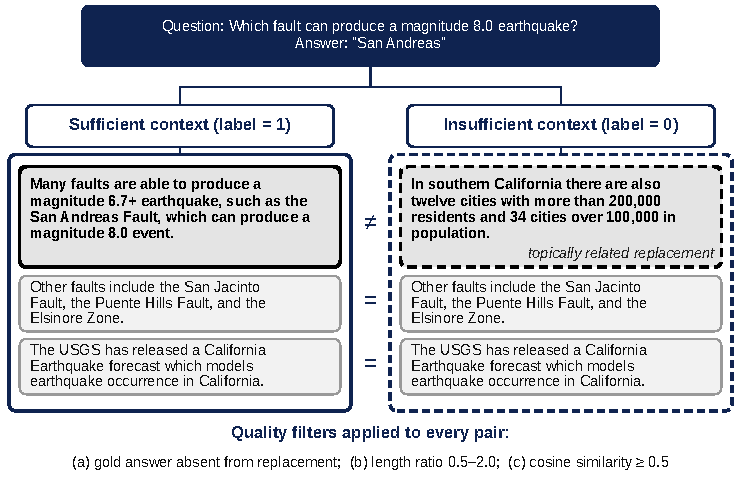
\includegraphics[width=0.76\textwidth]{Figure_2.pdf}
\caption{Paired construction example. The sufficient context (left) contains the answer-bearing sentence (highlighted). The insufficient context (right) replaces it with a topically similar sentence from a different passage. All three quality filters pass: no gold answer in the replacement sentence, length ratio within $[0.5, 2.0]$, cosine similarity $\geq 0.5$.}
\label{fig:construction}
\end{figure}

\subsection{Validity}
\label{sec:validity}

A benchmark of this kind can fail in four ways, and we test each one. First, the labels can be wrong. Eleven independent annotators judged 30 stratified pairs, seeing the question and the passage but not the gold answer (Appendix~\ref{sec:human_ann}). Agreement was moderate (Fleiss' $\kappa = 0.52$, 90.0\% majority-vote agreement with the labels), with disagreements concentrated in implicit-inference multi-hop and comparative items. Second, the labels can be right but learnable from surface features. In the HotpotQA distractor validation set (7,405 questions with 73,700 context paragraphs), the paragraphs that support the answer average 70 words against 95 for the distractors, and a logistic regression on passage length alone separates them at 0.649 AUROC under question-grouped cross-validation, with word and entity counts adding nothing (0.651). In \bench{} the sufficient-to-insufficient length ratio is $1.008 \pm 0.053$ in characters and $1.011 \pm 0.073$ in words, entity density is matched (0.174 against 0.170 capitalised tokens per word), and the same classifier scores 0.503 with length alone and 0.513 with all three features. Third, the conclusions can be fragile to residual label error. Flipping 5 to 20\% of test labels at random leaves the probe--VC gap $\geq 0.05$ on all three 7B--8B models (Appendix~\ref{sec:robustness}). Fourth, the construction can leave an artefact, since replacing one sentence may break the local coherence of the passage, and a reader trained on the benchmark could learn the edit rather than the missing answer. With random unrelated paragraphs as the insufficient class, probe AUROC is 0.99 for all three 7B--8B models, so the probes do not depend on a splice; two further controls measure how much they use it (Appendix~\ref{sec:robustness}, Table~\ref{tab:splice}). A probe trained on the hidden state of the context alone, with no question in the prompt, reaches 0.87--0.89 AUROC against 0.90--0.91 for the Standard probe: most of the separability is a property of the context text, and the question adds 0.06--0.09 on SQuAD and 0.01--0.02 on HotpotQA. We then apply the same edit to sufficient contexts, replacing a sentence far from the answer sentence with a pool sentence (1,038 test questions), and score the result with the benchmark-trained probes. On SQuAD, where the answer survives the edit, the mean probe score falls from 0.87--0.90 to 0.71--0.80, 14--27\% of the edited sufficient contexts fall below the decision threshold against 6--14\% of the originals, and edited sufficient contexts remain separable from insufficient ones at 0.85--0.87 AUROC. On HotpotQA, 40\% of the edits removed a supporting-fact sentence, and those contexts score close to insufficient ones, as they should; where the supporting facts survive, 29--42\% of edited contexts fall below threshold against 7--16\% of the originals, and the edited-versus-insufficient AUROC is 0.82--0.86. Adding edited sufficient training contexts, labelled sufficient, to the Llama probes reduces the share below threshold to 26--30\% at a cost of 0.05 AUROC on the original pairs. The edit is therefore a cue that a trained reader partly uses, and the benchmark AUROC of such a reader is an upper bound that includes it; the zero-shot predictors are not fitted to the benchmark, so part of the probe--output gap on \bench{} may reflect the cue, and the retrieved-context evaluation of Section~\ref{sec:retrieved}, where no context is edited, is the evidence for the ordering that is free of it. Because the answer filter applies to the replacement sentence only, the gold-answer string occurs somewhere in 9.0\% of insufficient test contexts (5.5\% at word boundaries, mostly subjective and factual items), in a sentence that does not answer the question, and an oracle that checks for the gold-answer string reaches 0.931 AUROC on the test split. These checks do not rule out semantic-overlap cues (embedding similarity reaches 0.634, Table~\ref{tab:main_results}) or address whether a model uses the context it is given (Section~\ref{sec:discussion}, Limitations).

The paired design also addresses the concern raised by \citet{magata2026answeronly} for hallucination probes, namely that separability can come from the answer tokens rather than the context. Our probes read the final token of the question-plus-context prompt before any answer is generated, and the two members of a pair share the question, so whatever separates them must come from the context.

PK rates on the test split under the first-sentence rule range from 5.1\% (Llama~3.1~8B) to 18.4\% (DeepSeek-R1-Distill~32B): Llama~3.1~8B 5.1\%, Mistral~7B 17.0\%, Qwen~2.5~7B 10.0\%, Qwen3~8B 13.3\%, Qwen~2.5~14B 7.0\%, and DeepSeek-R1-Distill~32B 18.4\% (under the original rule 2.2, 17.4, 3.9, 2.0, 3.6 and 18.2\%). The frontier models were scored under the original rule on the version 1.0 split (Appendix~\ref{sec:frontier_app}): Opus~4.7 35.0\% and GPT-5.5 29.7\%; their closed-book generations were not retained, so the first-sentence rule cannot be applied to them.

\section{Experimental Setup}
\label{sec:methods}

\subsection{Predictors and Controls}
\label{sec:methods_detection}

We evaluated 18 predictors across five families (listed in full in Table~\ref{tab:main_results}), grouped by where each reads from the transformer. \textit{Hidden-state probes} read the last-token residual stream, using either $\mathbf{h}(q{+}c)$ directly (Standard) or $\mathbf{h}(q{+}c) - \mathbf{h}(q)$ to isolate the context contribution (CSP, Context Subtraction Probe), each in linear (LogReg) and neural (MLP) variants; the layer is selected on the validation split (Appendix~\ref{sec:layers}). The \textit{mechanistic} methods read attention. ReDeEP \citep{sun2025redeep} decomposes attention into External Context Score (ECS) and Parametric Knowledge Score (PKS), reported separately and combined, and the Lookback Lens \citep{chuang2024lookback} computes, for every head, the share of attention mass that generated tokens send back to the context, then classifies those per-head ratios with a logistic regression trained on the \bench{} training split. The \textit{sampling-based internal} method INSIDE \citep{chen2024inside} draws 10 continuations per item and scores the differential entropy of their hidden-state covariance (EigenScore), read at the probe layer (checked in Appendix~\ref{sec:robustness}). \textit{Generation-based} methods include verbalized confidence (VC), VC under the model's chat template, the probability the model assigns to answering yes to the sufficiency question, read from the next-token logits ($P(\text{Yes})$), semantic entropy \citep{farquhar2024semantic}, token entropy, and two oracle methods that see the gold answer. \textit{Behavioural} methods include LLM self-judge and embedding similarity. Prompt templates are given in Appendix~\ref{sec:prompts}. AUROC \citep{hanley1982meaning} is the primary metric, being threshold-free and comparable across methods whose scores live on incomparable scales; gate accuracy and gated answer accuracy are reported in Section~\ref{sec:sprobe_results}.

Two controls address the asymmetry that the probes are trained on the benchmark whereas the output-based methods are zero-shot. First, a \emph{trained output readout}: a logistic regression on the per-example output-based scores of each model, fitted and evaluated on the test split by five-fold cross-validation grouped by question, once with the non-oracle scores (verbalized confidence and the $P(\text{Yes})$ logit, each under the plain and the chat-template prompt; verbalized comparison, in which the model answers with and without the context and rates from 0 to 100 how much the context changed its answer; and response delta, the cosine similarity between the embeddings of its answers with and without the context) and once adding the oracle token-probability delta, the gain in log-probability of the gold answer when the context is added. The two contrastive scores are not among the 18 predictors of Table~\ref{tab:main_results}; they are included here so that the readout sees every output-based signal we computed. The probes are evaluated under the same folds. Second, \emph{leave-one-source-out transfer}: the probe is trained on the training split with one source dataset removed and tested on that source's test questions, and compared with the probe trained on the full training split and with zero-shot verbalized confidence on the same questions.

\subsection{Models}
\label{sec:models}

\textit{Small open-weight (7B--8B)}: Llama~3.1~8B Instruct \citep{grattafiori2024llama}, Mistral~7B Instruct~v0.3 \citep{jiang2023mistral}, and Qwen~2.5~7B Instruct \citep{qwen2024}, loaded in 8-bit quantisation (a bfloat16 comparison is in Appendix~\ref{sec:robustness}); the three were developed and trained independently. \textit{Recent open-weight}: Qwen3~8B \citep{qwen3}, a 36-layer model released in 2025 and trained with a native thinking mode; as the most recent open-weight release in the same size class, it separates training recipe from scale, and it is also evaluated with thinking enabled (Appendix~\ref{sec:thinking_app}). \textit{Medium (14B--32B)}: Qwen~2.5~14B Instruct \citep{qwen2024} in 8-bit and DeepSeek-R1-Distill~32B \citep{deepseekai2025r1} in 4-bit NF4 quantisation, each evaluated with the full pipeline. \textit{Frontier API}: Claude Opus~4.7 and GPT-5.5, evaluated on output-based methods only (white-box access unavailable), with chain-of-thought (CoT) prompting evaluated on Opus~4.7.

\subsection{Standalone Encoder and Long-Context Extension}
\label{sec:sufficiencyprobe}

The \sprobe{} operationalises the same delta construction as the CSP probe inside a 395M ModernBERT-large \citep{warner2024modernbert} encoder rather than the base LLM: it encodes the (question, context) pair and the question alone, takes the difference of their \texttt{[CLS]} representations, and passes it through a linear classifier, so no LLM is needed at inference. It is trained on coverage pairs (a passage containing the gold answer and the same passage with the answer-bearing sentence deleted) built from open-domain QA datasets, with every \bench{} test question excluded. The \emph{cross-source} variant is trained on TriviaQA and NQ (788 pairs), two datasets that do not appear in \bench{}; the \emph{cross-dataset} variant adds HotpotQA coverage pairs (1,715 pairs in total); the \emph{in-distribution} variant adds the \bench{} training and validation splits (3,067 training and 944 validation pairs, the latter the 528 \bench{} validation examples plus 416 coverage pairs). Decision thresholds are selected on the \bench{} validation split, so gate accuracy and the downstream figures for this tier assume access to a small labelled sample from the target construction, whereas the AUROC figures do not. Training details, an out-of-distribution SciQ set, and two LLM-free reference classifiers are described in Appendix~\ref{sec:sprobe_app}.

The long-context extension asks whether a detector can still tell that a passage suffices once it is buried among thousands of tokens of unrelated text. We extended the paired construction to 4,000, 16,000, 32,000 and 100,000 tokens (about six to 150 pages, against a few hundred tokens for one retrieved passage). For each of 300 test questions, stratified by type, a haystack is built from the sufficient contexts of other training-split questions, excluding any passage that contains the gold answer or overlaps the target context; the target passage, in its sufficient or its insufficient version, is inserted at the first, middle or last position, balanced across questions, and the same haystack serves both conditions. Llama~3.1~8B and Qwen~2.5~7B were run to 100,000 tokens (Qwen with YaRN scaling \citep{peng2024yarn}) and Mistral~7B to 16,000, because the next length exceeds its 32,768-token window once tokenised by its own tokenizer and the model exposes no rope scaling; a nested subset of 150 questions (probes) and 100 (VC) is used at 100,000 tokens because of cost. We evaluate the \emph{transfer} probe, the CSP probe trained on short contexts and applied unchanged at the same layer, the \emph{in-distribution} probe, trained on the long-context set by 5-fold cross-validation grouped by question, and verbalized confidence with the same prompt. Further details are in Appendix~\ref{sec:longcontext_app}.

\section{Results}
\label{sec:results}

\subsection{Detection Performance by Access Point}
\label{sec:main_results}

\begin{figure}[t]
\centering
\Description{Dot-and-range chart of AUROC for sixteen predictors on three models, sorted by mean AUROC, with hidden-state probes above output-based methods.}
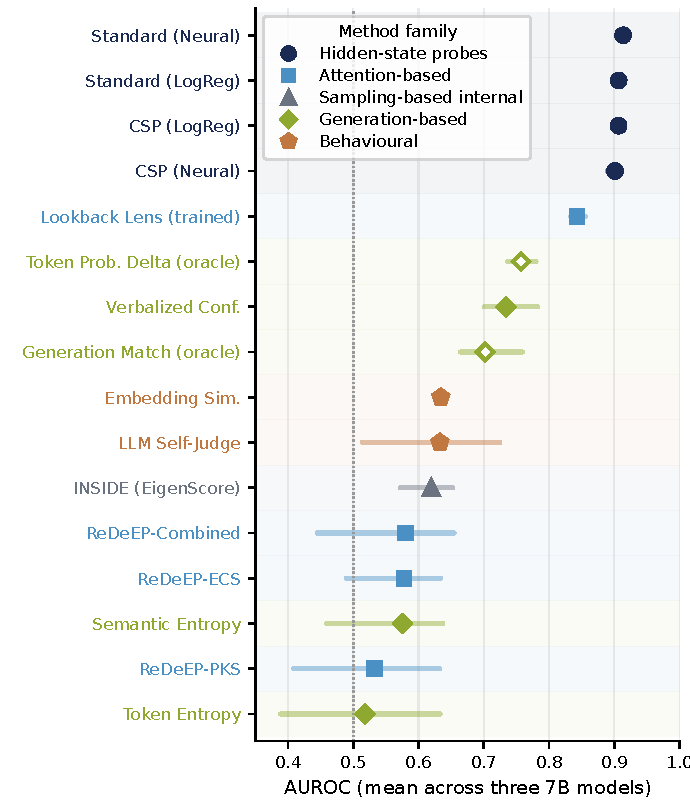
\includegraphics[width=0.71\textwidth]{Figure_4.pdf}
\caption{AUROC on the \bench{} test split for the 16 predictors of the main comparison across the three 7B-class open-weight models (the two zero-shot output readouts added last, $P(\text{Yes})$ and verbalized confidence under the chat template, appear in Table~\ref{tab:main_results} only). Methods are sorted by mean AUROC. The dot is the mean across the three models, the bar is the range across them, and colour denotes the method family. Open markers are oracle methods that require the gold answer.}
\label{fig:main_comparison}
\end{figure}

\begin{table}[t]
\centering
\caption{Sufficiency prediction AUROC on the \bench{} test split with 95\% CIs (question-clustered bootstrap for the logistic probes, verbalized confidence and the two logit/template readouts, which resamples both conditions of a question together; Hanley--McNeil for the other rows). Paired tests are reported in the text. Best per model in \textbf{bold}. $^*$Requires oracle gold-answer access. $^\dagger$Trained on the \bench{} training split, like the probes.}
\label{tab:main_results}
\small
\begin{tabular}{@{}lccc@{}}
\toprule
Method & Mistral 7B & Llama 3.1 8B & Qwen 2.5 7B \\
\midrule
\multicolumn{4}{l}{\textit{Hidden-state probes}} \\
  Standard (LogReg) & 0.910$\pm$0.012 & 0.907$\pm$0.012 & 0.904$\pm$0.012 \\
  CSP (LogReg) & 0.902$\pm$0.013 & 0.904$\pm$0.012 & \textbf{0.914}$\pm$0.012 \\
  Standard (Neural) & \textbf{0.915}$\pm$0.012 & \textbf{0.919}$\pm$0.012 & 0.907$\pm$0.013 \\
  CSP (Neural) & 0.911$\pm$0.013 & 0.890$\pm$0.014 & 0.902$\pm$0.013 \\
\midrule
\multicolumn{4}{l}{\textit{Mechanistic (attention-based)}} \\
  ReDeEP-ECS & 0.610$\pm$0.024 & 0.634$\pm$0.023 & 0.490$\pm$0.024 \\
  ReDeEP-PKS & 0.557$\pm$0.024 & 0.633$\pm$0.023 & 0.409$\pm$0.024 \\
  ReDeEP-Combined & 0.655$\pm$0.023 & 0.641$\pm$0.023 & 0.445$\pm$0.024 \\
  Lookback Lens$^\dagger$ & 0.833$\pm$0.014 & 0.855$\pm$0.014 & 0.840$\pm$0.015 \\
\midrule
\multicolumn{4}{l}{\textit{Sampling-based internal}} \\
  INSIDE (EigenScore) & 0.653$\pm$0.019 & 0.572$\pm$0.023 & 0.635$\pm$0.020 \\
\midrule
\multicolumn{4}{l}{\textit{Generation-based}} \\
  VC & 0.701$\pm$0.022 & 0.719$\pm$0.022 & 0.782$\pm$0.019 \\
  VC, chat template & 0.710$\pm$0.016 & 0.770$\pm$0.016 & 0.748$\pm$0.015 \\
  $P(\text{Yes})$ logit & 0.770$\pm$0.015 & 0.806$\pm$0.014 & 0.819$\pm$0.015 \\
  Token Entropy & 0.633$\pm$0.023 & 0.533$\pm$0.024 & 0.389$\pm$0.024 \\
  Token Prob.\ Delta$^*$ & 0.780$\pm$0.020 & 0.754$\pm$0.020 & 0.737$\pm$0.021 \\
  Generation Match$^*$ & 0.759$\pm$0.020 & 0.665$\pm$0.023 & 0.683$\pm$0.022 \\
  Semantic Entropy & 0.637$\pm$0.023 & 0.630$\pm$0.023 & 0.459$\pm$0.024 \\
\midrule
\multicolumn{4}{l}{\textit{Behavioural}} \\
  LLM Self-Judge & 0.659$\pm$0.023 & 0.514$\pm$0.024 & 0.725$\pm$0.021 \\
  Embedding Similarity & 0.634$\pm$0.023 & 0.634$\pm$0.023 & 0.634$\pm$0.023 \\
\bottomrule
\end{tabular}
\end{table}

\paragraph{Paired tests.}
Because the two conditions of a question are paired, per-example intervals understate the uncertainty and unpaired comparisons waste the pairing. We therefore recomputed, from the stored per-example scores, question-clustered bootstrap intervals (2,000 resamples) and paired bootstrap differences between predictors on every open-weight model with stored scores. The Standard probe exceeds verbalized confidence by 0.12 (Qwen~2.5~7B and 14B) to 0.21 (Mistral~7B) AUROC, with every clustered 95\% interval excluding zero and Holm-corrected $p \leq 0.003$ within each model, the floor set by 2,000 resamples; the Standard and CSP probes differ by at most 0.010 AUROC, in either direction depending on the model. The clustered intervals are within 0.001 of the Hanley--McNeil intervals, so the pairing does not change the width of the intervals in Table~\ref{tab:main_results}, only the validity of the comparison. Within the PK$=$0 stratum the differences are the same to within 0.01. The script and full tables are released with the code.


The separation between access points is visible in Figure~\ref{fig:main_comparison} and quantified in Table~\ref{tab:main_results}. All four probe variants achieve 0.890--0.919 AUROC. On these three models, every zero-shot method that reads the model's output achieves at most 0.821 AUROC, so on every model the weakest probe exceeds the strongest non-oracle output-based method, by 0.08 on Llama~3.1~8B and Qwen~2.5~7B and by 0.13 on Mistral~7B, and the paired 95\% intervals of the probe--confidence difference exclude zero on every model (paired tests below). Neural probes are within 0.015 AUROC of their linear counterparts in either direction. Among the readouts of generated text, verbalized confidence is the strongest (0.701--0.782); the logit readout $P(\text{Yes})$ is better still, at 0.770--0.819 ($+$0.04 to $+$0.09 over verbalized confidence, paired CIs excluding zero; 0.774--0.821 under the chat template), whereas the chat template changes verbalized confidence by $+$0.01 on Mistral~7B, $+$0.05 on Llama~3.1~8B and $-$0.03 on Qwen~2.5~7B, so prompt format does not explain the ceiling. ReDeEP, despite reading from every attention head across all layers, does not exceed it with either of its hand-designed scores, and neither of the two oracle methods that see the gold answer exceeds the 0.82 that the best zero-shot output readout reaches. Semantic entropy and token entropy score at most 0.64, and below chance on Qwen~2.5~7B.

\paragraph{Access-point ordering with the readout held fixed.}
The two detectors from the literature that read internal state isolate the access point from the readout. INSIDE reaches 0.572--0.653 AUROC, no better than verbalized confidence. The Lookback Lens, a logistic regression on per-head attention ratios trained on the same split as the probes, reaches 0.833--0.855. Holding the readout fixed as a trained linear classifier across the two internal access points, attention therefore reaches 0.833--0.855 and the residual stream 0.902--0.914, while nothing read zero-shot from the output exceeds 0.821. A layer sweep is consistent with this ordering: the Standard linear probe placed on the final layer, where the representation is about to become output, falls to 0.82--0.86 on the four open-weight models with a full sweep (Appendix~\ref{sec:layers}), 0.06 to 0.08 below its selected layer and roughly the level of the attention readout, although we did not run a paired per-example test across layers.

\paragraph{Supervision does not close the gap.}
Under five-fold cross-validation grouped by question, a logistic regression on the six non-oracle output scores reaches 0.75--0.81 AUROC, within 0.02 of the best zero-shot output readout, and adding the oracle token-probability delta lifts it to 0.84--0.86 (Appendix~\ref{sec:robustness}, Table~\ref{tab:controls}). The Standard and CSP probes under the same folds reach 0.89--0.91. With supervision matched and oracle information allowed, the gap is 0.04 to 0.08 rather than the 0.12 to 0.21 of the zero-shot comparison, and without oracle information it is 0.09 to 0.17.

\paragraph{Frontier models.}
Claude Opus~4.7 achieves 0.802 overall VC AUROC, but 35.0\% of its test examples are PK$=$1, inflating this figure. At PK$=$0, Opus~4.7 VC falls to 0.774 and GPT-5.5 VC to 0.742 (Table~\ref{tab:scale}, Appendix~\ref{sec:frontier_app}). CoT prompting of the Opus~4.7 judge achieves 0.729, 0.012 above the same judge without CoT (0.717). Both are far below the accuracy that \citet{joren2025sufficient} report for their autorater on their own data, where an insufficient context is a different document and length differs between the classes; on matched pairs the same judgement is harder, which is what the construction is for. Even the highest frontier score (0.802) is 0.09--0.12 below the open-weight 7B probes, and enabling the native thinking mode of a small open-weight model does not change this picture (Appendix~\ref{sec:thinking_app}).

\paragraph{Gap by question type.}
The probe--VC gap is smallest on factual questions and largest on comparative ones (Table~\ref{tab:per_qtype}), at $+$0.154 on factual, $+$0.200 on multi-hop, $+$0.245 on subjective, and $+$0.360 on comparative. The probe holds between 0.91 and 0.94 on the three extractive types, so the differences come from verbalized confidence, which falls from 0.76 on factual to 0.56 on comparative questions. Of the under-confident VC errors, 97.6\% have confidence exactly 0, and 88.2\% of the over-confident ones exceed 0.8, so its errors are extreme rather than borderline. VC correlates only weakly with context length (Spearman $\rho = 0.14$ to $0.21$ across the three models).

\begin{table}[t]
\centering
\begin{minipage}[t]{0.40\textwidth}
\centering
\caption{Per-type AUROC for Mistral~7B. PRW = fraction of test items where the Standard probe is correct and VC is wrong, both at a threshold of 0.5.}
\label{tab:per_qtype}
\footnotesize
\begin{tabular}{@{}lcccc@{}}
\toprule
Type & Probe & VC & $\Delta$ & PRW \\
\midrule
  Factual     & 0.917 & 0.762 & $+$0.154 & 16\% \\
  Multi-hop   & 0.936 & 0.735 & $+$0.200 & 21\% \\
  Comparative & 0.915 & 0.555 & $+$0.360 & 33\% \\
  Subjective  & 0.832 & 0.587 & $+$0.245 & 31\% \\
\bottomrule
\end{tabular}
\end{minipage}\hfill
\begin{minipage}[t]{0.58\textwidth}
\centering
\caption{Probe (CSP LogReg) and VC AUROC by model and scale. PK$=$0 is computed under the first-sentence rule (Section~\ref{sec:construction}) and shown where the PK rate is $\geq 5\%$; --- where not measured. $^\ddagger$Verbalized confidence from the chat prompt without thinking (Appendix~\ref{sec:thinking_app}), the Qwen3 variant with PK-stratified scores; the raw-prompt value is 0.729 (Section~\ref{sec:scale_transfer}). $^\dagger$Output-based methods only, scored on the version 1.0 test split (Appendix~\ref{sec:frontier_app}).}
\label{tab:scale}
\footnotesize
\begin{tabular}{@{}llcccc@{}}
\toprule
Model & Size & Probe & VC & Probe PK$=$0 & VC PK$=$0 \\
\midrule
Llama 3.1         & 8B  & 0.904 & 0.719 & 0.903 & 0.716 \\
Mistral           & 7B  & 0.902 & 0.701 & 0.896 & 0.695 \\
Qwen 2.5          & 7B  & 0.914 & 0.782 & 0.911 & 0.778 \\
Qwen3             & 8B  & 0.918 & 0.781$^\ddagger$ & ---   & 0.775$^\ddagger$ \\
Qwen 2.5          & 14B & 0.949 & 0.818 & 0.949 & 0.817 \\
DeepSeek-R1-Dist. & 32B & 0.946 & 0.803 & 0.947 & 0.803 \\
\midrule
Claude Opus~4.7$^\dagger$ & --- & --- & 0.802 & --- & 0.774 \\
GPT-5.5$^\dagger$         & --- & --- & 0.752 & --- & 0.742 \\
\bottomrule
\end{tabular}
\end{minipage}
\end{table}

\subsection{Scale, Model Generation and Source Transfer}
\label{sec:scale_transfer}

Probe AUROC rises from 0.90--0.92 in the 7B--8B class to 0.95 at 14B and 32B, and verbalized confidence rises from 0.70--0.78 to 0.80--0.82 (Table~\ref{tab:scale}), so the gap at the larger sizes, 0.13 to 0.14, sits inside the 0.13 to 0.20 of the 7B--8B class and does not close. With two models in the larger class, one of them a reasoning-distilled model, we read this as a bound on what scale alone changes rather than as a trend. Qwen3~8B shows the same pattern: the Standard probe reaches 0.922 AUROC with logistic regression (0.918 for the CSP probe) and 0.934 with a neural classifier, against 0.729 for verbalized confidence on the raw prompt, 0.510 for token entropy, and 0.750 for generation match, with a PK rate of 13.3\% under the first-sentence rule (2.0\% under the original rule).

The probe's advantage is largest in distribution (Appendix~\ref{sec:robustness}, Table~\ref{tab:loso}). Trained on the full training split, the Standard probe scores 0.93--0.94 on the HotpotQA test questions, 0.91--0.92 on SQuAD, and 0.76--0.83 on ELI5 for the three 7B--8B models. Trained with one source held out, it loses 0.03 to 0.05 AUROC on SQuAD and 0.08 to 0.10 on HotpotQA and ELI5: 0.83--0.86 on HotpotQA, 0.87--0.89 on SQuAD, and 0.66--0.74 on ELI5. Against zero-shot verbalized confidence on the same questions, the held-out probe keeps a margin on every source, of 0.03 to 0.13 on SQuAD, 0.04 to 0.14 on HotpotQA, and 0.05 to 0.16 on ELI5. The CSP probe behaves the same way. Together with the long-context results of Section~\ref{sec:longcontext}, this bounds the probe advantage: it is largest when the probe is trained on the target construction and source, and it shrinks, without vanishing, as the test distribution moves away.

\subsection{Sufficiency Prediction on Retrieved Contexts}
\label{sec:retrieved}
The benchmark fixes the context so that the confounds cannot act. A RAG system, however, receives whatever the retriever returns, so we repeat the comparison on retrieved contexts. We index the 66,581 distinct paragraphs of the HotpotQA distractor validation set with BM25 \citep{robertson2009bm25} (Lucene via Pyserini \citep{lin2021pyserini}, $k_1 = 0.9$, $b = 0.4$) and retrieve the top-$k$ paragraphs for each question; the context is the concatenation of the retrieved paragraphs in rank order, each preceded by its title, and it is sufficient when every gold-support paragraph of the question is among them. Every question is two-hop, so no context is sufficient at $k = 1$; 33\% are at $k = 3$, 44.5\% at $k = 5$ and 59\% at $k = 10$, and we use $k = 5$, which gives contexts of about 700 tokens. We draw 3,000 training and 1,500 test questions from the validation set, disjoint from each other and from every \bench{} question. Three families of predictor, and a supervised text-only reference, are compared: the retriever-score predictors of post-retrieval QPP (top-1 score, score gap between ranks 1 and 2, mean, sum and standard deviation of the top-$k$ scores, the last an unnormalised form of normalised query commitment (NQC) \citep{shtok2012predicting}, and a logistic regression over the five, fitted on the training questions), the standard post-retrieval predictors weighted information gain (WIG) \citep{zhou2007query}, NQC \citep{shtok2012predicting}, score magnitude and variance (SMV) \citep{tao2014smv}, clarity \citep{cronentownsend2002predicting} and the maximum standard deviation $\sigma_{\max}$ \citep{perez2010stddev}, computed from the Lucene index with the collection treated as one document for the corpus score, at $k = 5$, 10 and 20, with a logistic regression over the five at the $k$ selected by cross-validation on the training questions ($k = 10$), with the cosine similarity between E5 embeddings \citep{wang2022e5} of the question and the context as a dense counterpart; verbalized confidence and the model's decision to answer rather than abstain; the Standard and CSP probes, first transferred from \bench{} at their selected layers without retraining, then retrained on the 3,000 retrieved training contexts with the recipe of Section~\ref{sec:methods}; and, as a supervised text-only reference, the \sprobe{} encoder of Section~\ref{sec:sufficiencyprobe}, transferred from \bench{} and retrained on the same 3,000 contexts (binary cross-entropy, 10\% of the training questions held out for early stopping, 512- and 1,024-token windows; the contexts average 680 tokens). Parametric knowledge is scored per question with the first-sentence rule of Section~\ref{sec:construction}; 6.5\% of the test questions are answered closed-book by Llama, 25.5\% by Mistral and 11.4\% by Qwen. CIs and paired tests are question-clustered bootstraps as in Section~\ref{sec:main_results}.

\begin{table}[t]
\caption{Sufficiency prediction on BM25-retrieved contexts (top-5 passages, pooled HotpotQA paragraphs; 1,500 test questions, 44.5\% sufficient). AUROC with 95\% question-clustered bootstrap CI (2,000 resamples; 1,000 for the text-only encoder). Transferred probes are the \bench{}-trained probes at their selected layers, applied without retraining; retrained probes are trained on 3,000 disjoint retrieved contexts with the same recipe. Retriever-score, similarity and text-only encoder predictors do not read the generator, so one value spans the model columns; every other predictor reads the listed model. The sum of the top-$k$ scores is rank-equivalent to their mean at fixed $k$ and is omitted from the table but included in the regression.}
\label{tab:retrieved}
\footnotesize
\setlength{\tabcolsep}{4pt}
\begin{tabular}{lccc}
\toprule
Predictor & Llama~3.1~8B & Mistral~7B & Qwen~2.5~7B \\
\midrule
\multicolumn{4}{l}{\emph{Retriever scores (post-retrieval QPP)}} \\
Top-1 BM25 score & \multicolumn{3}{c}{0.568 [0.539, 0.598]} \\
Score gap (rank 1 $-$ rank 2) & \multicolumn{3}{c}{0.496 [0.467, 0.524]} \\
Mean top-$k$ score & \multicolumn{3}{c}{0.572 [0.542, 0.602]} \\
Std.\ dev.\ of top-$k$ scores (unnorm.\ NQC) & \multicolumn{3}{c}{0.584 [0.555, 0.612]} \\
Logistic regression over the five & \multicolumn{3}{c}{0.671 [0.643, 0.699]} \\
SMV at $k = 10$ (best standard predictor) & \multicolumn{3}{c}{0.614 [0.584, 0.643]} \\
Logistic regression, five standard predictors ($k = 10$) & \multicolumn{3}{c}{0.655 [0.626, 0.683]} \\
\multicolumn{4}{l}{\emph{Query--context similarity}} \\
E5 cosine (question, context) & \multicolumn{3}{c}{0.712 [0.687, 0.738]} \\
\multicolumn{4}{l}{\emph{Output-based}} \\
Verbalized confidence & 0.707 [0.684, 0.729] & 0.617 [0.594, 0.641] & 0.700 [0.674, 0.724] \\
Model does not abstain & 0.725 [0.702, 0.747] & 0.664 [0.643, 0.684] & 0.735 [0.711, 0.758] \\
\multicolumn{4}{l}{\emph{Hidden-state probes, transferred from \bench{}}} \\
Standard probe & 0.807 [0.785, 0.829] & 0.773 [0.750, 0.795] & 0.811 [0.789, 0.832] \\
CSP probe & 0.795 [0.772, 0.817] & 0.747 [0.724, 0.773] & 0.818 [0.797, 0.839] \\
\multicolumn{4}{l}{\emph{Hidden-state probes, retrained on retrieved contexts}} \\
Standard probe & 0.936 [0.923, 0.947] & 0.916 [0.902, 0.929] & 0.936 [0.923, 0.946] \\
CSP probe & 0.924 [0.911, 0.936] & 0.906 [0.890, 0.920] & 0.935 [0.923, 0.946] \\
\multicolumn{4}{l}{\emph{Text-only encoder (\sprobe{}, 395M, no LLM)}} \\
Transferred from \bench{} & \multicolumn{3}{c}{0.786 [0.762, 0.809]} \\
Retrained, 512-token window & \multicolumn{3}{c}{0.921 [0.907, 0.934]} \\
Retrained, 1,024-token window & \multicolumn{3}{c}{0.953 [0.942, 0.962]} \\
\bottomrule
\end{tabular}
\end{table}

On retrieved contexts the supervised readers again lead (Table~\ref{tab:retrieved}). The retriever scores alone predict sufficiency poorly: no single score exceeds 0.584 AUROC, the score gap is at chance, and the logistic regression over the five reaches 0.671, slightly below the E5 similarity at 0.712. The standard predictors do no better: SMV at $k = 10$ is the best of them at 0.614, clarity is at chance (0.48--0.49 at every $k$), and the logistic regression over the five standard predictors reaches 0.655; the transferred Standard probe exceeds each of them by 0.12 to 0.34 AUROC on every model (paired $\Delta$, Holm-corrected $p = 0.009$ over the 18 comparisons per model). Verbalized confidence scores 0.617--0.707 and the model's decision to answer 0.664--0.735. The probes transferred from \bench{} without any training on retrieved contexts score 0.747--0.818, above verbalized confidence by 0.09 to 0.16 AUROC on every model (paired $\Delta$ with 95\% CI excluding zero; bootstrap $p < 0.001$, at most 0.003 after Holm correction over the six probe-versus-confidence comparisons, the floor of 2,000 resamples). They also exceed the E5 similarity and the retriever-score regression on every model (paired $\Delta$ of $+$0.06 to $+$0.11 against E5 and $+$0.08 to $+$0.15 against the regression, Holm-corrected $p \leq 0.004$ over the eight comparisons per model, except the transferred CSP probe on Mistral against E5, $\Delta = +0.036$ [0.001, 0.070], $p = 0.043$). The probes retrained on retrieved contexts score 0.906--0.936, at or above the 0.89--0.92 the same probes reach on the benchmark. A supervised text-only encoder is at least as good: the \sprobe{} trained on the benchmark transfers at 0.786, within the range of the transferred LLM probes, and retrained on the same 3,000 retrieved contexts it reaches 0.921 with a 512-token window, which truncates 81\% of the contexts, and 0.953 with a 1,024-token window, above the retrained Standard probes by 0.017 to 0.037 (paired $\Delta$, $p \leq 0.012$). On retrieved contexts, then, the margin over the output-based predictors is a property of supervised reading, whether of the generator's state or of the text, and not of the residual stream as such; what the hidden-state probe adds is that it needs no second model and reads the generator whose answer is being gated (Section~\ref{sec:discussion}). Unlike on the benchmark, where embedding similarity scores 0.634, an unsupervised generator-free signal is competitive with the output: the E5 similarity matches or exceeds verbalized confidence on every model, and on Mistral the retriever-score regression does too. The ordering among the three families is the same within the stratum of questions the model cannot answer closed-book (PK = 0), where the transferred Standard probe scores 0.809 on Llama, 0.771 on Mistral and 0.807 on Qwen, so parametric knowledge does not account for the margin, and it is unchanged when the title prefixes are removed from the retrieved context (transferred probes move by at most 0.008). In the risk--coverage view, the area under the risk--coverage curve (AURC) is 0.32--0.37 for the transferred probes against 0.43--0.46 for verbalized confidence, and 0.24--0.26 for the retrained probes; at 10\% risk, verbalized confidence cannot cover any question on any model, while a retrained probe covers 29--37\%. One quantity that verbalized confidence predicts better than the probes is the model's own answer quality: its Kendall $\tau$ with answer F1 is higher than that of the transferred probes on Llama and Mistral (0.47 against 0.35 on Llama; Qwen's answers are too often not short-form for the comparison to be informative), because confidence and answer are read from the same generation, whereas the probe is trained on the sufficiency label and does not see whether the model will use the context (Limitation 5).

Gold-support containment is a conservative label. Among the contexts it marks insufficient, 37\% contain the gold answer string, usually because another retrieved paragraph repeats the fact that the missing support paragraph would have provided, and an answer-string containment label agrees with it on 79\% of the 1,413 questions whose answer is not yes or no. Restricting to the 1,110 questions where the two labels agree raises the generator-based predictors and the retriever-score regression, leaves the similarity baseline within 0.01, and leaves the ordering unchanged: retriever-score regression 0.680, E5 similarity 0.704, verbalized confidence 0.646--0.745, transferred Standard probe 0.805--0.850, retrained Standard probe 0.943--0.963. Under the answer-string label alone (1,413 non-yes/no questions) the ordering also holds, with transferred probes at 0.734--0.776 and verbalized confidence at 0.612--0.690. Finally, a layer sweep of the retrained Standard probe peaks at layer 14 to 15 of 32 on Llama and Mistral (0.936 and 0.933) and at layer 19 of 28 on Qwen (0.936), and falls to 0.834--0.866 at the final layer, the profile of Appendix~\ref{sec:layers} on retrieved contexts.

\subsection{Deployment Tiers}
\label{sec:sprobe_results}

A deployed gate answers only when the predictor is confident, so the operating quantity is the risk--coverage trade-off of selective answering \citep{kamath2020selective}: the fraction of questions answered against the fraction of those answers given on insufficient context. From the stored test scores, the probes cover 31--48\% of questions at a risk of 10\% and 7--35\% at 5\%, depending on the model, whereas verbalized confidence, whose scores are concentrated on a few values, cannot reach either risk level on any model; the area under the risk--coverage curve is 0.19--0.22 for the probes and 0.27--0.36 for verbalized confidence. The detectors also differ in what they need at inference time, which determines where each can be deployed (Table~\ref{tab:deployment}). Verbalized confidence needs a full generation, the CSP probe one forward pass with white-box access to the residual stream, and the \sprobe{} no LLM at all. Trained on TriviaQA and NQ with no \bench{} exposure, the cross-source \sprobe{} achieves 0.769 AUROC (factual 0.856, multi-hop 0.865, comparative 0.833, subjective 0.672). Without running any LLM it is within 0.013 of the best 7B-class VC baseline (Qwen~2.5~7B, 0.782) and matches the PK$=$0 verbalized confidence of Opus~4.7 (0.774). Adding HotpotQA coverage pairs lifts it to 0.870, with the gain concentrated on the multi-hop items (0.961) that share that source. Two LLM-free classifiers give the tier a reference point: an off-the-shelf SQuAD~v2 answerability model, DeBERTa-v3-large \citep{he2023debertav3}, reaches 0.794 AUROC on the test split, and MiniCheck \citep{tang2024minicheck}, given the gold answer, reaches 0.884 but is an oracle (Appendix~\ref{sec:sprobe_app}).

At the threshold $t = 0.67$ selected on the validation split, the cross-source \sprobe{} achieves 70.0\% gate accuracy on the test set. In a quadrant-balanced Mistral~7B gating simulation on 296 test examples, it achieves 72.3\% answer accuracy, above the no-gate baseline (46.3\%) and the VC gate (68.6\%) but below the CSP probe (77.7\%), with the oracle gate at 88.5\%. Trained in distribution, the \sprobe{} reaches 0.966 AUROC on the test split, 91.2\% gate accuracy and 81.4\% answer accuracy in the gating simulation, and transfers without further training to the SciQ set at 0.958 AUROC (the cross-source variant reaches 0.933 there); the paragraph-sharing check for this variant is in Appendix~\ref{sec:sprobe_app}.

\begin{table}[t]
\centering
\caption{Deployment tier comparison. AUROC on the \bench{} test split ($n{=}2{,}138$). Downstream acc.\ = answer accuracy of Mistral~7B in a quadrant-balanced gating simulation on 296 test examples, with each gate applied to the same generations. ``gen.''$=$full autoregressive decoding; ``fwd.''$=$one forward pass. The last two rows are LLM-free reference classifiers. $^\ddagger$AUROC from Qwen~2.5~7B, the strongest 7B VC and its CSP probe; downstream accuracy from the Mistral~7B simulation, where the probe gate is Mistral's CSP logistic probe. $^*$Requires the gold answer.}
\label{tab:deployment}
\small
\begin{tabular}{@{}lcccc@{}}
\toprule
Method & AUROC & Downstream acc. & Latency & LLM? \\
\midrule
No gate (always answer) & --- & 46.3\% & --- & --- \\
VC (open-weight 7B)$^\ddagger$ & 0.782 & 68.6\% & ${\sim}500$\,ms & gen. \\
VC (Opus~4.7, frontier, v1.0 split) & 0.802 & --- & ${\sim}1\,000$\,ms & gen. \\
CSP probe (Qwen~2.5~7B)$^\ddagger$ & 0.914 & 77.7\% & ${\sim}100$\,ms & fwd. \\
\sprobe{} (cross-source)       & 0.769 & 72.3\% & 7.3\,ms & none \\
\sprobe{} (cross-dataset)      & 0.870 & 73.3\% & 7.3\,ms & none \\
\sprobe{} (trained in distribution) & 0.966 & 81.4\% & 7.3\,ms & none \\
SQuAD~v2 answerability (DeBERTa) & 0.794 & --- & --- & none \\
MiniCheck (gold answer)$^*$   & 0.884 & --- & --- & none \\
\bottomrule
\end{tabular}
\end{table}

\subsection{Sufficiency Detection at Long Context}
\label{sec:longcontext}


Figure~\ref{fig:longcontext} (Appendix~\ref{sec:longcontext_app}) reports AUROC as a function of context length, with the values in Table~\ref{tab:longcontext}. On the original passages the transfer probe reproduces the main result at 0.90--0.93 AUROC against 0.71--0.79 for verbalized confidence. Once the passage is embedded in a haystack every final-token readout weakens, but not equally: at 4,000 tokens, about ten passages, the transfer probe falls to 0.72--0.79, the in-distribution probe to 0.79--0.85 and verbalized confidence to 0.58--0.73, each drop larger than the width of the 95\% bootstrap interval except for verbalized confidence on Qwen, and the decline continues with length; at 100,000 tokens the transfer probe is at 0.51--0.61, the in-distribution probe at 0.57--0.74 and verbalized confidence at 0.59--0.61. A probe retrained at the target length stays above verbalized confidence by 0.09 to 0.24 AUROC up to 32,000 tokens for every model and by 0.14 on Llama at 100,000 tokens; Qwen at 100,000 tokens is the one cell where it falls below (0.574 against 0.593). The probe trained on short contexts keeps a margin of 0.06 to 0.14 at 4,000 tokens, but from 16,000 tokens on it is within 0.02 of verbalized confidence or below it, except Mistral at 16,000 tokens (0.618 against 0.522); the Standard probe behaves like the CSP probe throughout. Two observations locate the loss. In a layer sweep on the long-context set the best-scoring layer moves two to three blocks deeper at 16,000 tokens, where it yields 0.69--0.72 for the transfer probe and 0.81--0.84 for the in-distribution probe, so part of the drop at the fixed layer is relocation of the signal rather than its disappearance; and at 16,000 tokens the in-distribution probe reaches 0.83--0.89 when the target passage is last in the haystack, 0.75--0.83 when first and 0.71--0.75 when in the middle (Appendix~\ref{sec:longcontext_app}). The extension therefore bounds the main result to retrieved contexts of a few hundred tokens: once the passage is buried, a final-token readout of any kind is a weak instrument, and the natural next step is a readout over passage positions.

\section{Discussion}
\label{sec:discussion}

\paragraph{Interpretation of the ceiling.}
The ceiling is a statement about access to the evaluated model's own state. It rises by at most 0.04 from 7B to the largest models we test, by 0.04 to 0.09 when the output is read from the next-token logits rather than from the generated text, is unaffected by chain-of-thought prompting, and is not a bound on the task itself, since a separately trained answerability classifier with no access to the model reaches 0.794, the level of the best zero-shot output readout (0.77--0.82), and a text-only encoder trained on the same labels matches or exceeds the probe (Section~\ref{sec:retrieved}). What a detector can recover depends on where it reads: on the three models where all three access points were measured, attention yields less than the residual stream with the classifier type held fixed, and nothing read from the output reaches either; the layer sweep, a supporting analysis rather than a localisation, is consistent with the residual-stream signal being degraded by the time the output is prepared. Supervision does not explain the gap, since a readout trained on the output-based scores stays near the zero-shot ceiling without oracle information and reaches 0.84--0.86 with it, against 0.89 to 0.91 for the probe under the same protocol. Distribution partly does: on a held-out source dataset the probe loses 0.03 to 0.10 AUROC while keeping a margin over verbalized confidence on every source, and at long context the probe trained on short passages loses most of its margin. Construction partly does too: the benchmark edit is a cue that trained readers use (Section~\ref{sec:validity}), which is why the unedited retrieved contexts carry the ordering. The ceiling is therefore a statement about what zero-shot reading of the output exposes of a signal that supervised readouts, of the residual stream or of the text itself, recover; whether a generator fine-tuned to report sufficiency would recover it too is untested (Limitation 7), the probe reads the signal reliably only in distribution, and the residual-stream readout is itself a bounded instrument.

Several smaller observations are consistent with this reading. On Mistral~7B, steering along the probe direction moves abstention in the direction the sign predicts (Appendix~\ref{sec:steering_app}). INSIDE, which scores the spread of sampled outputs in hidden-state space, performs like an output-based method, since its signal is still a property of the outputs. Neural probes are within 0.015 AUROC of linear ones, so little of the signal requires a non-linear readout. That prompted CoT adds only 0.012 AUROC on Opus~4.7, and that the native thinking mode of Qwen3~8B adds nothing over the same instruction without it, agree with reports that stated reasoning can rationalise an answer driven by factors the explanation never mentions \citep{turpin2023unfaithful}: deliberation at the output stage cannot expose a signal that the output stage does not read. Prior output-based methods report AUROC above 0.78 on their own hallucination- and correctness-detection benchmarks, whereas on \bench{} verbalized confidence achieves 0.70--0.82, the $P(\text{Yes})$ logit readout 0.77--0.82, and the other zero-shot output-based methods less. Because the two sets of numbers come from different pipelines, models and source data, we do not attribute the difference to confound removal alone; the within-pipeline evidence is that passage length alone separates gold from distractor paragraphs at 0.65 AUROC in uncontrolled HotpotQA and scores at chance here.

\paragraph{Relation to query performance prediction.}
QPP and sufficiency prediction estimate adjacent quantities from different evidence. Post-retrieval QPP reads the ranked list, so it can be computed for any generator, and it predicts whether the evidence is there; sufficiency prediction asks whether the retrieved evidence lets the question be answered, and the predictors compared here read either the generator or the text. On retrieved contexts (Section~\ref{sec:retrieved}), retriever-score and similarity predictors recover part of the label without reading the generator (0.67--0.71 AUROC), and supervised readers of the question and the passages together, the hidden-state probe or the text-only encoder, recover more. \citet{dado2026benefit} report the opposite ordering for the benefit of retrieval: their supervised post-generation predictor stays ahead of a probe that adapts the final hidden states. The two results do not conflict. Their output predictor is trained and reads the generated answer, whereas the output predictors compared here are zero-shot, and their probe reads the final layer, where our sweep finds the weakest sufficiency signal (Appendix~\ref{sec:layers}). Our contribution is to show, on data where length and prior knowledge cannot explain the result, that the gap between zero-shot output readouts and a trained intermediate-layer readout is not explained by a trained readout of the output scores and is consistent with an access limit.

\paragraph{Relevance under long-context models.}
Context windows have grown by two orders of magnitude since RAG was introduced, which raises the objection that sufficiency detection matters less when a model can read a whole document collection at once. Section~\ref{sec:longcontext} answers in two parts. Sufficiency detection does not become easier: once the relevant passage is embedded among distractors every method degrades, and longer contexts are likely to strengthen the confound we control for, since the presence of any text suppresses abstention \citep{joren2025sufficient}. And the access-limit result applies to retrieved-passage contexts of a few hundred tokens. A final-token readout of any kind is weak in long contexts, and the recency effect indicates that the problem becomes one of localisation, which suggests reading the residual stream at the passage positions instead; the position effect combines a recency advantage with the mid-context trough reported for long-context question answering \citep{liu2024lost}.

\paragraph{Practical implications.}
A deployed gate operates at one threshold, so the practical quantities are gate accuracy and the answer accuracy of the gated system (Table~\ref{tab:deployment}). For the cross-source \sprobe{} gate accuracy (70.0\%) is bounded by its AUROC (0.769), yet the gate is still useful (72.3\% answer accuracy against 46.3\% without one). With the threshold set on the validation split of the target construction, as for every variant here, the AUROC ranking carries over into decisions (Table~\ref{tab:deployment}). The practical question for a deployed gate is then whether white-box access is available, in which case the CSP probe adds 0.11--0.12 AUROC over the off-the-shelf answerability classifier, and otherwise whether matched-pair training data exist for a standalone encoder.

\paragraph{Limitations.}
Ten limitations restrict the scope of these conclusions. First, label validation rests on 30 human-annotated pairs; majority-vote agreement with the labels is 90.0\%, but agreement among annotators is moderate ($\kappa = 0.52$), driven by implicit-inference multi-hop and comparative items, and it is the four automatic checks of Section~\ref{sec:validity} and the automatically labelled SciQ document-swap set (Appendix~\ref{sec:sprobe_app}) that make the conclusions independent of those 30 pairs. Second, HotpotQA supplies 55\% of the questions, so the aggregate AUROC weights the source on which the probes score highest; the per-source numbers of Section~\ref{sec:scale_transfer} are the ones to compare across sources. Third, all evaluation is on English text from Wikipedia, Reddit and science textbooks; clinical and legal retrieval, where a missed insufficiency is most costly, are untested. Fourth, the main benchmark uses single-passage contexts of a few hundred tokens; the long-context extension bounds the result, but it covers a single readout position and two models to 100,000 tokens. Fifth, sufficiency is necessary but not sufficient for a correct answer; whether the model uses the context it is given is the grounding problem, which our labels do not address. Sixth, the frontier models were scored without their native reasoning modes, and the CSP probe cannot be applied to them, so the frontier evidence bears on the output-based ceiling only; prompted CoT adds 0.012 AUROC on Opus~4.7 and 0.021 on Qwen3~8B, native thinking on Qwen3~8B adds nothing, and a frontier run with reasoning enabled is the direct follow-up. Seventh, the three access points are compared through readouts that differ in input dimensionality, readout position and supervision; the dimension-matched probes of Appendix~\ref{sec:robustness} (Table~\ref{tab:dimension}) show that input size alone does not produce the ordering, but the comparison remains one of readouts as deployed; no generator fine-tuned to report sufficiency was evaluated, so an elicitation failure that fine-tuning would repair is not excluded, and the steering experiment is reported with the random-direction control of Appendix~\ref{sec:steering_app}; the supervision asymmetry, by contrast, is addressed by the trained output readout of Section~\ref{sec:main_results}. Eighth, the retrieved-context validation of Section~\ref{sec:retrieved} uses one lexical retriever over one paragraph pool, and its sufficiency labels follow from gold-support containment rather than from a human judgment of the concatenated context; a dense retriever and an open corpus are the natural extensions. Ninth, the probe's advantage is largest in distribution: a deployment that cannot train on the target source or construction should expect the held-out numbers of Section~\ref{sec:scale_transfer}, and the \sprobe{} and the answerability classifier cover black-box deployments at the AUROC reported in Table~\ref{tab:deployment}, below the probe without in-distribution training data and above it with such data. Tenth, the edit that creates an insufficient context is itself a cue: a probe on the context alone reaches 0.87--0.89 AUROC and edited-but-sufficient contexts lose part of their score (Section~\ref{sec:validity}), so the benchmark AUROC of any reader trained on it, probe or text-only encoder, includes the cue; the ordering of access points rests on the unedited retrieved contexts, where the probes keep their advantage over the output-based predictors.

\section{Conclusion}
\label{sec:conclusion}

Deciding whether retrieved context suffices is a performance-prediction problem at the generation stage, and how well it can be solved depends on where the predictor reads. On a benchmark in which the passage-length and parametric-knowledge confounds are removed by construction, no zero-shot predictor that reads a model's output, including a logit readout, reaches 0.83 overall AUROC, while a linear probe on the residual stream reaches 0.90--0.95. The gap survives every model family and scale we test and is not closed by training a readout on the output-based scores, and on the three models where all three access points were measured, detection improves in the order outputs, attention, residual stream. The ceiling is an access limit, and it persists on BM25-retrieved contexts against the retriever-score predictors of query performance prediction. It is also bounded: the probe loses 0.03 to 0.10 AUROC on a held-out source dataset, and when the same passages are embedded in 4,000 to 100,000 tokens the transferred probe and verbalized confidence fade alike, a probe retrained at the target length keeps a margin that narrows with length and closes in one cell at 100,000 tokens, and at 16,000 tokens every readout depends strongly on where the passage sits, so the next step is a readout over passage positions. When matched-pair training data from the target construction exist, a standalone encoder trained on them is at least as accurate as the CSP probe (0.966 against 0.914 on the benchmark, 0.953 against 0.936 on retrieved contexts) and needs no access to the generator; the CSP probe is the choice when white-box access is available and no second model is wanted, and even an off-the-shelf answerability classifier already matches the zero-shot verbalized confidence of the 7B models. The benchmark, the evaluation pipeline and the probe training code are publicly available (see Data Availability).

\begin{acks}
We thank the 11 annotators who took part in the benchmark validation study; the study collected only their sufficiency judgments on passage pairs and no personal data. During the preparation of this work the authors used Claude (Anthropic) to assist with language editing and manuscript formatting, and to assist in writing parts of the analysis and plotting code; the authors reviewed and verified all such output against the underlying data and take full responsibility for the content. This research did not receive any specific grant from funding agencies in the public, commercial, or not-for-profit sectors.
\end{acks}

\section*{Data Availability}
\bench{} (version 1.1), the evaluation pipeline and the code that trains and scores the probes are available at \url{https://github.com/inab-lab/SufficiencyBench}. The three \sprobe{} checkpoints (cross-source, cross-dataset and in-distribution) are published as release assets of the same repository, with a loading example in its README.

\bibliographystyle{ACM-Reference-Format}
\bibliography{references,ir_references}

\clearpage
\appendix

\section{The \texorpdfstring{2$\times$2}{2x2} Design}
\label{sec:design_fig}
\begin{figure}[h]
\centering
\Description{Two-by-two grid of sufficiency against parametric knowledge defining the quadrants Q1 to Q4.}
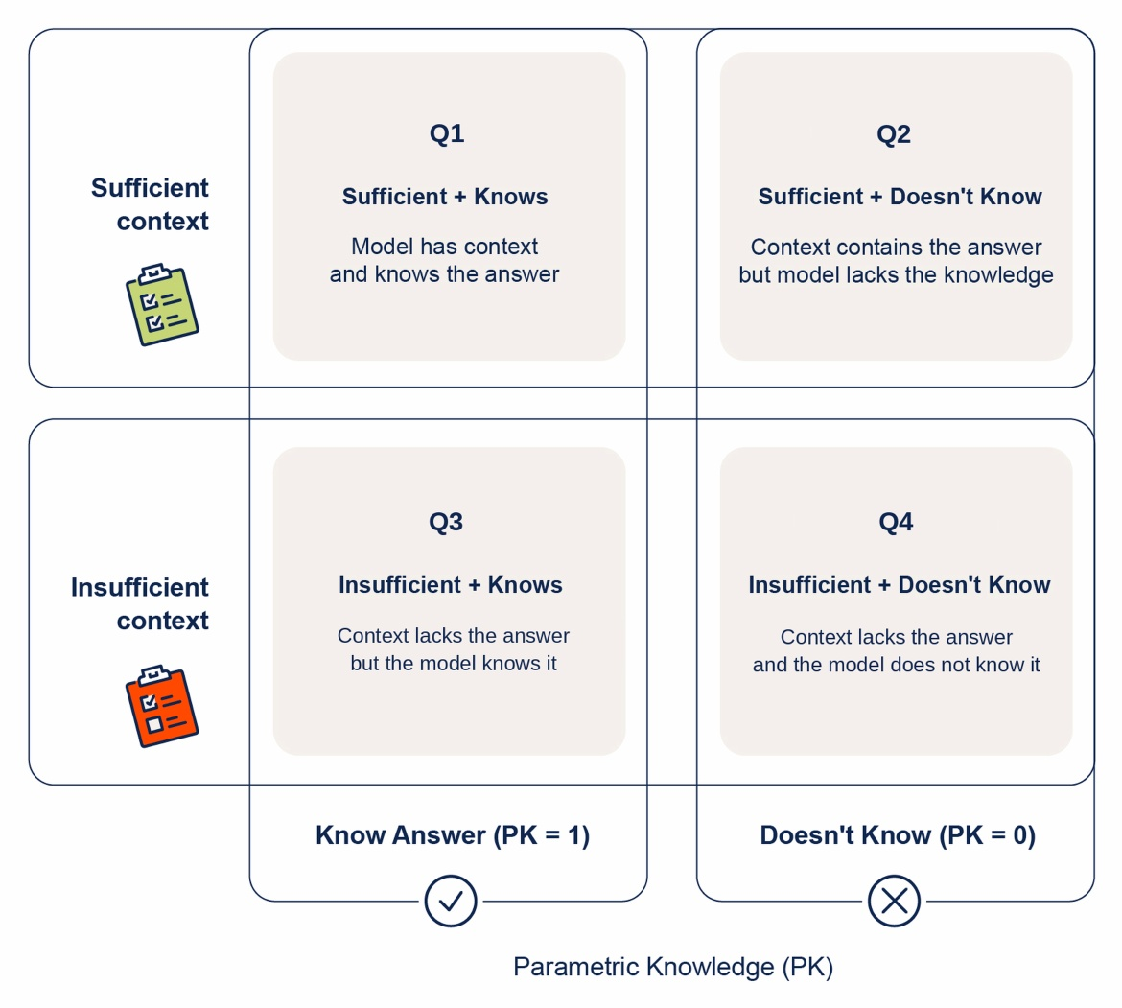
\includegraphics[width=0.6\textwidth]{Figure_1.pdf}
\caption{The 2$\times$2 design of \bench{}. Sufficiency (Y-axis) is model-agnostic. PK (X-axis) is per-model, determined via closed-book evaluation. Q3 is the critical quadrant where parametric knowledge and an insufficient context are expected to pull an output-based score in opposite directions.}
\label{fig:framework}
\end{figure}

\section{Human Annotation Protocol}
\label{sec:human_ann}
Thirty stratified pairs were judged by 11 independent annotators, who saw the question and the passage but not the gold answer and were asked whether the passage alone was sufficient to answer the question without external knowledge. Majority-vote agreement was 90.0\% and Fleiss' $\kappa = 0.52$. The 10\% disagreements involved borderline implicit-inference cases in multi-hop and comparative types.

\section{Whitespace Artefact}
\label{sec:whitespace}
A construction artefact was found during a leakage audit and removed before the main results were computed; the frontier-model runs and the chunked-prefill control (Appendix~\ref{sec:robustness}) predate the fix. In the first version of the benchmark the sufficient contexts kept the double spaces that follow sentence boundaries in the source passages, whereas the edited insufficient contexts were re-joined with single spaces. The number of double spaces alone separated the two conditions at 0.775 AUROC overall and 0.991 on the HotpotQA items, and every tokeniser used here emits a distinct token for a double space, so the hidden-state probes could read the cue. With whitespace collapsed in both conditions, the Standard probe of the three 7B--8B models fell from 0.930--0.934 to 0.904--0.910 AUROC, with the loss confined to the HotpotQA items (multi-hop and comparative, 0.98--0.99 to 0.93--0.94), while the factual items rose by about 0.05 and the subjective items changed by less than 0.02. The output-based methods were unaffected: verbalized confidence scored 0.50 on pairs that differed only in whitespace, and every output-based method moved by less than 0.02 after normalisation. All results in this paper use the normalised benchmark (version 1.1). The frontier-model runs of Appendix~\ref{sec:frontier_app} predate the normalisation and were scored on the version 1.0 test split (1,112 questions); they are output-based and are reported as measured.

\section{Robustness Checks}
\paragraph{Parametric-knowledge rule.}
Two rules were applied to the same closed-book generations. The original rule counted a question as known if the normalised gold answer occurred anywhere in the 60-token generation and no abstention phrase occurred anywhere in it. Several models append an abstention phrase after a correct first sentence (``Sheldon Adelson. I don't know. Sheldon Adelson\ldots''), which the original rule scored as not known. The first-sentence rule used in the paper requires the gold answer in the first sentence and no abstention phrase in that sentence. On the test split it raises the PK rate from 2.2 to 5.1\% (Llama~3.1~8B), 3.9 to 10.0\% (Qwen~2.5~7B), 2.0 to 13.3\% (Qwen3~8B) and 3.6 to 7.0\% (Qwen~2.5~14B), and leaves Mistral~7B (17.4 to 17.0\%) and DeepSeek-R1-Distill~32B (18.2 to 18.4\%) essentially unchanged; between 4 and 125 questions flip per model, nearly all from PK$=$0 to PK$=$1 except on Mistral~7B, where 8 of the 12 flips go the other way. The first-sentence rule over-counts on comparison and yes/no questions, where the gold answer is one of the options named in the question and can appear in a first sentence that states the opposite, so comparative questions reach 54--56\% PK on Mistral and DeepSeek. Because PK$=$0 excludes every flagged question, over-counting makes that stratum more conservative, not less. The PK$=$0 AUROC of the CSP probe and of verbalized confidence changes by at most 0.003 between the two rules on every model, and the PK$=$1 stratum remains too small to compare the predictors on the four models with low PK rates. The recomputation script and both label sets are released with the code.

\label{sec:robustness}

\paragraph{Label noise.}
We randomly flipped test labels at rates of 5\%, 10\%, 15\%, and 20\% (500 resamples each). Probe AUROC degrades gracefully (from 0.904--0.910 to 0.742--0.746 at 20\% noise), but the probe--VC gap remains $\geq 0.09$ on Llama and Mistral and $\geq 0.05$ on Qwen~2.5~7B, whose verbalized confidence is the strongest, across all noise levels.

\paragraph{Supervision-matched and cross-source controls.}
Tables~\ref{tab:controls} and~\ref{tab:loso} give the per-model numbers behind Sections~\ref{sec:main_results} and~\ref{sec:scale_transfer}. The zero-shot verbalized-confidence values are recomputed from the per-example scores of the same run as Table~\ref{tab:main_results} and differ from it by at most 0.004.

\begin{table}[h]
\centering
\caption{Supervision-matched comparison on the test split, AUROC under five-fold cross-validation grouped by question. Non-oracle readout: verbalized confidence and $P(\text{Yes})$ logit under the plain and the chat-template prompt, verbalized comparison, response delta. With oracle: the same plus the token-probability delta, which requires the gold answer.}
\label{tab:controls}
\small
\begin{tabular}{lcccc}
\toprule
Model & Output readout (non-oracle) & Output readout (with oracle) & Standard probe & CSP probe \\
\midrule
Llama~3.1~8B & 0.814 & 0.855 & 0.900 & 0.904 \\
Mistral~7B & 0.749 & 0.839 & 0.915 & 0.903 \\
Qwen~2.5~7B & 0.806 & 0.852 & 0.900 & 0.892 \\
\bottomrule
\end{tabular}
\end{table}

\paragraph{Input dimensionality.} The trained output readout has six input scalars, the Lookback Lens about 1,000 per-head ratios and the residual-stream probe 3,584 to 4,096 dimensions, so the ordering of access points could reflect input size. Table~\ref{tab:dimension} reports the Standard and CSP probes at the selected layer after projecting the training-split states to $d$ dimensions by PCA (fitted on the training split) or by a Gaussian random projection, with the same standardisation and classifier. Three to four principal components already give 0.73--0.84 AUROC, above zero-shot verbalized confidence on every model, and at four components the better of the two probes matches or exceeds the best zero-shot output readout, $P(\text{Yes})$, on every model, 32 components reach 0.85--0.88, and 256 match the full state; a random 1,024-dimensional projection, the dimensionality of the Lookback Lens, scores 0.86--0.88 against its 0.83--0.86. The ordering therefore does not reduce to input dimensionality, although the comparison still differs in readout position and supervision (Limitation 7).

\begin{table}[h]
\centering
\caption{Standard / CSP probe AUROC at the selected layer as a function of input dimensionality $d$ (PCA fitted on the training split; RP = Gaussian random projection), test split, question-clustered bootstrap CIs within $\pm$0.015 throughout. Full = the probes of Table~\ref{tab:main_results}.}
\label{tab:dimension}
\footnotesize
\setlength{\tabcolsep}{3pt}
\begin{tabular}{lccccccc}
\toprule
$d$ & 3 & 4 & 32 & 256 & 1024 & RP 1024 & full \\
\midrule
Llama~3.1~8B & 0.784 / 0.733 & 0.794 / 0.826 & 0.865 / 0.867 & 0.910 / 0.905 & 0.881 / 0.882 & 0.861 / 0.856 & 0.907 / 0.904 \\
Mistral~7B & 0.773 / 0.765 & 0.790 / 0.806 & 0.846 / 0.870 & 0.910 / 0.907 & 0.881 / 0.880 & 0.867 / 0.857 & 0.910 / 0.902 \\
Qwen~2.5~7B & 0.834 / 0.833 & 0.838 / 0.841 & 0.877 / 0.868 & 0.908 / 0.907 & 0.879 / 0.889 & 0.871 / 0.875 & 0.904 / 0.914 \\
\bottomrule
\end{tabular}
\end{table}

\paragraph{Editing cue.} Table~\ref{tab:splice} gives the per-source numbers behind the fourth check of Section~\ref{sec:validity}. The context-only probe reads the last token of the prompt with the question line removed, at the Standard probe's layer. Edited sufficient contexts replace the non-answer sentence farthest from the answer sentence with the pool sentence closest in length, under the benchmark's filters; 31 of the 1,069 test questions had no admissible sentence. The decision threshold is the balanced-accuracy threshold of the validation split. On HotpotQA, 232 of the 574 edits replaced a supporting-fact sentence; restricted to the 342 that did not, 29--42\% of edited contexts fall below threshold (originals 7--16\%) and the edited-versus-insufficient AUROC is 0.82--0.86, whereas the edits that removed a supporting fact score close to insufficient contexts (0.60--0.66). The Llama probes retrained with 1,309 edited sufficient training contexts labelled sufficient reach 0.858 (Standard) and 0.853 (CSP) AUROC on the original test pairs, against 0.907 and 0.904, with 30\% and 26\% of edited contexts below threshold. The CSP probe behaves like the Standard probe throughout, and ELI5, where the probes are weakest, is the only source on which the context-only probe is not below the Standard probe.

\begin{table}[t]
\caption{Editing-cue controls on the test split, Standard probe. Context-only: probe on the hidden state of the context without the question. $p$: mean probe score of original sufficient (orig) and edited sufficient (edit) contexts; below thr.: share below the validation decision threshold; last column: AUROC of edited sufficient against insufficient contexts. Question-clustered bootstrap CIs (1,000 resamples; half-widths 0.01--0.04 for the AUROCs) are in the result files.}
\label{tab:splice}
\footnotesize
\setlength{\tabcolsep}{4pt}
\begin{tabular}{llccccccc}
\toprule
 & & \multicolumn{2}{c}{AUROC} & \multicolumn{2}{c}{$p$} & \multicolumn{2}{c}{Below thr.\ (\%)} & AUROC \\
\cmidrule(lr){3-4}\cmidrule(lr){5-6}\cmidrule(lr){7-8}
Model & Source & Context-only & Standard & orig & edit & orig & edit & edit vs.\ insuf. \\
\midrule
  Llama~3.1~8B & SQuAD & 0.844 & 0.917 & 0.900 & 0.796 & 7 & 14 & 0.873 \\
   & HotpotQA & 0.928 & 0.941 & 0.891 & 0.518 & 8 & 44 & 0.778 \\
   & ELI5 & 0.835 & 0.756 & 0.739 & 0.396 & 22 & 55 & 0.523 \\
   & All & 0.889 & 0.907 & 0.866 & 0.570 & 10 & 38 & 0.765 \\
  \addlinespace
  Mistral~7B & SQuAD & 0.859 & 0.917 & 0.868 & 0.714 & 6 & 19 & 0.847 \\
   & HotpotQA & 0.914 & 0.932 & 0.834 & 0.413 & 9 & 46 & 0.740 \\
   & ELI5 & 0.835 & 0.832 & 0.749 & 0.304 & 14 & 59 & 0.533 \\
   & All & 0.884 & 0.910 & 0.828 & 0.474 & 9 & 41 & 0.738 \\
  \addlinespace
  Qwen~2.5~7B & SQuAD & 0.815 & 0.908 & 0.872 & 0.755 & 14 & 27 & 0.859 \\
   & HotpotQA & 0.921 & 0.935 & 0.863 & 0.478 & 15 & 55 & 0.761 \\
   & ELI5 & 0.789 & 0.780 & 0.705 & 0.365 & 33 & 68 & 0.514 \\
   & All & 0.870 & 0.904 & 0.837 & 0.532 & 18 & 50 & 0.749 \\
\bottomrule
\end{tabular}
\end{table}



\begin{table}[h]
\centering
\caption{Leave-one-source-out transfer of the Standard probe. In-source: trained on the full training split. Held-out: trained on the training split without that source. VC: zero-shot verbalized confidence on the same test questions.}
\label{tab:loso}
\small
\begin{tabular}{llccc}
\toprule
Source & Model & VC (zero-shot) & Probe (in-source) & Probe (held-out) \\
\midrule
SQuAD~v2  & Llama~3.1~8B  & 0.760 & 0.917 & 0.889 \\
          & Mistral~7B    & 0.762 & 0.917 & 0.870 \\
          & Qwen~2.5~7B   & 0.851 & 0.908 & 0.879 \\
HotpotQA  & Llama~3.1~8B  & 0.732 & 0.941 & 0.858 \\
          & Mistral~7B    & 0.703 & 0.932 & 0.847 \\
          & Qwen~2.5~7B   & 0.793 & 0.935 & 0.833 \\
ELI5      & Llama~3.1~8B  & 0.608 & 0.756 & 0.659 \\
          & Mistral~7B    & 0.587 & 0.832 & 0.743 \\
          & Qwen~2.5~7B   & 0.622 & 0.780 & 0.697 \\
\bottomrule
\end{tabular}
\end{table}

\paragraph{Pipeline controls.}
Three implementation choices were checked against their alternatives. Loading the 7B models in 8-bit rather than bfloat16 changes probe AUROC by at most 0.004 on 200 examples. Reading INSIDE at the midpoint of the network rather than at the probe layer changes its AUROC by less than 0.01. Above 32,768 tokens the long-context prompt is prefilled in chunks of 8,192 tokens. On a 60-question control at 32,000 tokens run on the first version of the benchmark, where both paths fit in memory, chunked prefill and standard decoding gave the same parsed confidence score on 96\% of Llama conditions and 100\% of Qwen conditions, with AUROC of 0.675 against 0.667 and 0.622 against 0.622, and in the present run the two paths were checked again on four prompts per model and length and agreed on every one.

\paragraph{Leave-question-out cross-validation.}
To confirm the probe learns a context-level signal rather than per-question identity, we held out both the sufficient and insufficient context for each question together. Under five-fold cross-validation grouped by question, the Standard and CSP probes reach 0.89--0.91 AUROC, and grouping the folds by shared source paragraph instead changes the result by at most 0.006 on every model, so the paragraph-level sharing noted in Appendix~\ref{sec:sprobe_app} (test questions whose source paragraph also appears in the training split under a different question) does not favour the probes.

\section{Frontier Model Details}
\label{sec:frontier_app}
Table~\ref{tab:frontier} gives the full output-based results for the two frontier API models, including the LLM-judge and chain-of-thought rows that Table~\ref{tab:scale} omits.
\begin{table}[h]
\centering
\caption{Frontier API model AUROC. PK$=$0 is the uncontaminated estimate (PK rates: Opus~4.7 35.0\%, GPT-5.5 29.7\%). These runs predate the whitespace normalisation (Appendix~\ref{sec:whitespace}) and were scored on the version 1.0 test split (1,112 questions). They are output-based, and every output-based method moved by less than 0.02 AUROC under normalisation, so they are reported as measured.}
\label{tab:frontier}
\small
\begin{tabular}{@{}llccc@{}}
\toprule
Model & Method & Overall & PK$=$0 & PK$=$1 \\
\midrule
Claude Opus~4.7 & VC           & 0.802 & 0.774 & 0.851 \\
                & LLM Judge    & 0.717 & 0.695 & 0.757 \\
                & CoT Judge    & 0.729 & ---   & ---   \\
\midrule
GPT-5.5         & VC           & 0.752 & 0.742 & 0.763 \\
                & LLM Judge    & 0.727 & 0.711 & 0.765 \\
\bottomrule
\end{tabular}
\end{table}

\section{\sprobe{} Details}
\label{sec:sprobe_app}
All three \sprobe{} variants use a pairwise contrastive loss plus binary cross-entropy for 10 epochs with model selection on validation AUROC. Their decision thresholds are selected on the \bench{} validation split by maximising balanced accuracy ($t = 0.67$, $0.12$, and $0.62$ for the cross-source, cross-dataset and in-distribution variants respectively), a single fixed threshold per variant used for all downstream evaluation. Besides the \bench{} test split, the variants are evaluated on an out-of-distribution set built from SciQ \citep{welbl2017sciq}, a science-textbook question answering dataset, with a document-swap construction rather than the sentence-level edit of \bench{}: each of 824 questions is paired with two contexts, its own support passage and the BM25 top-ranked support passage of a different question, filtered to exclude the answer, so this set does not control passage length.

The in-distribution \sprobe{} reaches 0.966 AUROC on the \bench{} test split (factual 0.964, multi-hop 0.979, comparative 0.987, subjective 0.909). Because SQuAD paragraphs carry several questions each, 56 test questions share their source paragraph with a different question in the training data. Excluding them leaves the AUROC at 0.965 (factual 0.958). On the SciQ set, the in-distribution variant reaches 0.958 AUROC and 90.2\% gate accuracy and the cross-source variant 0.933 and 78.9\%.

Two LLM-free classifiers give the standalone tier a reference point. An off-the-shelf SQuAD~v2 answerability model, DeBERTa-v3-large \citep{he2023debertav3} with 435M parameters scored by the margin between its best answer span and its no-answer logit, reaches 0.794 AUROC on the test split (factual 0.917, multi-hop 0.808, comparative 0.757, subjective 0.558). MiniCheck \citep{tang2024minicheck}, an entailment model given the gold answer as the claim, reaches 0.884.

\section{Long-Context Details}
\label{sec:longcontext_app}
Haystacks are nested, lengths are measured with the Llama tokeniser, the prompt template is unchanged, and Qwen~2.5~7B is run beyond its native window with YaRN scaling by a factor of four. The transfer probe is the CSP probe trained on the short-context training split at the layer selected on the validation split (Appendix~\ref{sec:layers}) and applied unchanged. The in-distribution probe is trained and evaluated on the long-context set itself by 5-fold cross-validation grouped by question, at the same layer. Verbalized confidence uses the same prompt and greedy decoding as before. Above 32,768 tokens the prompt is prefilled in chunks of 8,192 tokens to fit in memory, a path validated against standard decoding on a 60-question control (Appendix~\ref{sec:robustness}). Hidden states are read at the final token through forward hooks, without storing the full sequence, and confidence intervals are bootstrapped over questions.

\begin{figure}[t]
\centering
\Description{Line chart of AUROC against context length for the transferred probe, the retrained probe and verbalized confidence, with bootstrap bands, on three models.}
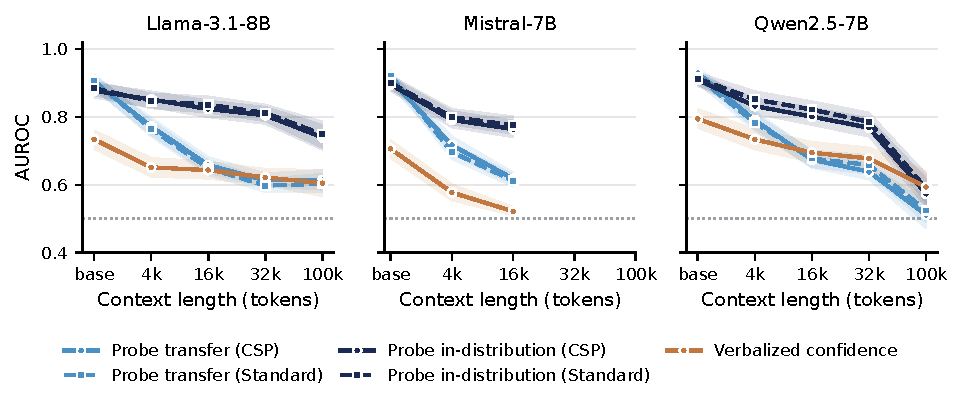
\includegraphics[width=\textwidth]{Figure_5.pdf}
\caption{AUROC as a function of context length for the transfer probe, the in-distribution probe, and verbalized confidence, with 95\% bootstrap bands over questions. Solid lines are the CSP probe and dashed lines the Standard probe. Mistral stops at 16k tokens because the next length exceeds its 32k window in its own tokenizer. The underlying values are in Table~\ref{tab:longcontext}.}
\label{fig:longcontext}
\end{figure}


In the layer sweep on the long-context set, the best-scoring layer of the Standard probe moves from blocks 13 to 17 on the original passages to 16 to 19 for the in-distribution probe at 16,000 tokens. By position, at 16,000 tokens the transfer probe shows the same split as the in-distribution probe (0.68--0.74 when the target passage is last against 0.56--0.68 elsewhere). At 100,000 tokens on Llama the last position still yields 0.78 for the in-distribution probe and 0.68 for the transfer probe, while at the first and middle positions the transfer probe is within 0.10 of chance.

\begin{table}[h]
\centering
\caption{AUROC on the long-context extension. Transfer = CSP probe trained on short contexts and applied unchanged. In-dist.\ = CSP probe trained by 5-fold grouped cross-validation at the same length. VC = verbalized confidence. Base = original passages. 300 questions per cell up to 32k tokens, and at 100k tokens 150 questions for the probes and 100 for VC. 95\% bootstrap intervals over questions in Figure~\ref{fig:longcontext}.}
\label{tab:longcontext}
\small
\begin{tabular}{@{}llccc@{}}
\toprule
Model & Context & Transfer & In-dist. & VC \\
\midrule
Llama 3.1 8B  & base & 0.902 & 0.877 & 0.734 \\
              & 4k   & 0.772 & 0.851 & 0.651 \\
              & 16k  & 0.658 & 0.823 & 0.643 \\
              & 32k  & 0.613 & 0.805 & 0.622 \\
              & 100k & 0.614 & 0.740 & 0.605 \\
\midrule
Mistral 7B    & base & 0.910 & 0.895 & 0.706 \\
              & 4k   & 0.717 & 0.791 & 0.577 \\
              & 16k  & 0.618 & 0.764 & 0.522 \\
\midrule
Qwen 2.5 7B   & base & 0.929 & 0.909 & 0.794 \\
              & 4k   & 0.790 & 0.832 & 0.734 \\
              & 16k  & 0.674 & 0.801 & 0.695 \\
              & 32k  & 0.638 & 0.768 & 0.678 \\
              & 100k & 0.511 & 0.574 & 0.593 \\
\bottomrule
\end{tabular}
\end{table}

\section{Prompt Templates}
\label{sec:prompts}

\paragraph{Verbalized confidence (open-weight models).}
\begin{quote}\small
Given the following context and question, answer only with a number from 0 to 100 representing how confident you are that the context contains enough information to answer the question (0 = definitely not, 100 = definitely yes). Output only the number.\\
Context: \{context\}\\
Question: \{question\}\\
Confidence:
\end{quote}

\paragraph{Verbalized confidence (frontier / API models).}
\begin{quote}\small
You are an expert judge. Given a context and a question, rate your confidence that the context alone is sufficient to answer the question. Respond with a single integer from 0 to 100. No explanation.\\
Context: \{context\}\\
Question: \{question\}
\end{quote}

\section{Layer Sweep}
\label{sec:layers}
For the four open-weight models with a full sweep, the layer of the Standard probe selected on the validation split lies between 41\% and 68\% of network depth (layer 14 of 32 for Llama~3.1~8B, 13 of 32 for Mistral~7B, 19 of 28 for Qwen~2.5~7B, and 20 of 36 for Qwen3~8B) and falls to 0.82--0.86 at the final layer (Figure~\ref{fig:layers}, Table~\ref{tab:layers}); on Qwen~2.5~7B the validation-selected layer sits one block past the test plateau. The drop from the selected to the final layer, 0.06 to 0.08 AUROC, is several times the width of the bootstrap interval, but we did not run a paired per-example test across layers. We read the sweep as consistent with the sufficiency direction being mixed into output-preparation computations in the final layers, and not as a precise localisation. A paired comparison of per-example scores across layers would settle the point and requires no new data.

Figure~\ref{fig:layers} shows the test AUROC of the Standard logistic-regression probe at every layer. Layer indices are zero-based block outputs, as in the released code (Data Availability), and depth is the index divided by the number of blocks. The layer used in the main results is the one with the highest validation AUROC. The signal is present from the first third of the network onwards, is strongest in the middle layers, and declines over the last third. The selected-layer values here are the Standard logistic-regression values of Table~\ref{tab:main_results} for the three 7B--8B models and of Section~\ref{sec:scale_transfer} for Qwen3~8B.

\begin{table}[h]
\centering
\caption{Layer sweep summary. Selected = layer with the highest validation AUROC (index / number of blocks, depth). Plateau = layers whose test AUROC is within 0.01 of the model's maximum.}
\label{tab:layers}
\small
\begin{tabular}{lcccc}
\toprule
Model & Selected layer & AUROC at selected & AUROC at final layer & Plateau \\
\midrule
Llama~3.1~8B  & 14/32 (44\%) & 0.907 & 0.847 & 12--14 \\
Mistral~7B  & 13/32 (41\%) & 0.910 & 0.827 & 12--16 \\
Qwen~2.5~7B  & 19/28 (68\%) & 0.904 & 0.822 & 17--18 \\
Qwen3~8B  & 20/36 (56\%) & 0.922 & 0.860 & 19--21 \\
\bottomrule
\end{tabular}
\end{table}

\begin{figure}[h]
\centering
\Description{Line chart of Standard probe AUROC against relative layer depth for each model, with the selected layer marked.}
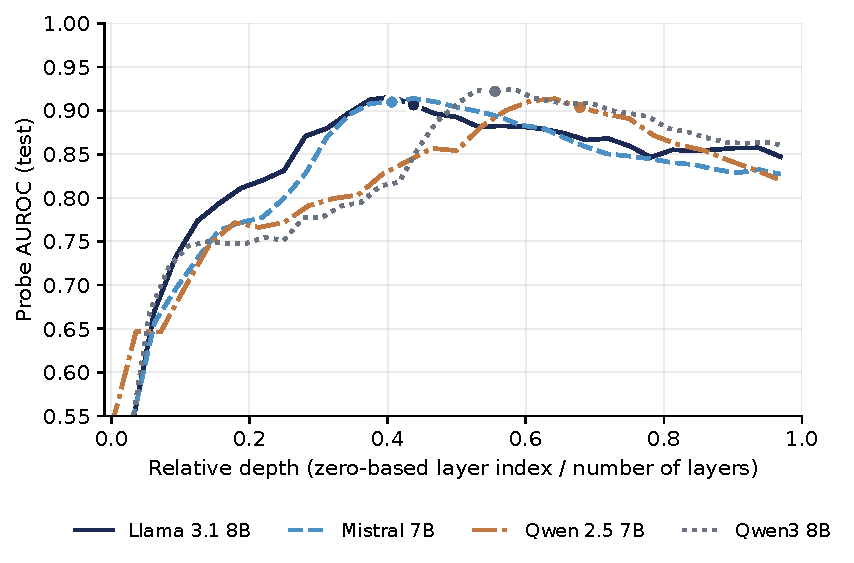
\includegraphics[width=0.72\textwidth]{Figure_D1.pdf}
\caption{Standard probe AUROC on the \bench{} test split as a function of relative depth. Markers show the layer selected on the validation split for each model.}
\label{fig:layers}
\end{figure}

\section{Activation Steering}
\label{sec:steering_app}
The probe results show where in the network the sufficiency signal can be read, but not that the model uses the direction the probe reads. To test this we steered Mistral~7B along the CSP probe direction and measured the effect on generation. The unit-norm coefficient vector of the layer-13 CSP probe, the layer selected on validation, was added to the residual stream at layers 11 to 15 during generation, scaled by $\alpha \times 0.15$ of the live residual-stream norm, with $\alpha \in \{-2, -1, 0, 1, 2\}$. Negative $\alpha$ pushes the representation towards the insufficient pole and positive $\alpha$ towards the sufficient pole. We evaluated 50 test items per quadrant of the 2$\times$2 design and recorded answer correctness and abstention, comparing each steered condition with $\alpha = 0$ by Fisher's exact test. Figure~\ref{fig:steering} plots, for each steering coefficient, the fraction of correct answers (top) and the abstention rate (bottom), with one line per quadrant.

Steering towards the insufficient pole at $\alpha = -1$ raises the abstention rate on insufficient contexts from 30\% to 60\% when the model knows the answer (Q3) and from 22\% to 70\% when it does not (Q4), while correctness on sufficient contexts with parametric knowledge (Q1) falls from 90\% to 74\%. Relative to $\alpha = 0$ the rise in abstention is significant in every quadrant (Fisher's exact test, $p = 0.015$ on Q1 and $p < 0.005$ on the other three). Steering towards the sufficient pole at $\alpha = 1$ lowers abstention on the insufficient quadrants from 30\% to 14\% (Q3) and from 22\% to 18\% (Q4) and leaves Q1 correctness within 6 points of the unsteered value. The effect is larger towards the insufficient pole than towards the sufficient one. At $|\alpha| = 2$ generation collapses in both directions, with correctness at or below 22\% and, towards the sufficient pole, abstention at zero. The collapse at $|\alpha| = 2$ is examined with the control below.

\paragraph{Random-direction control.} To separate the effect of the probe direction from generic perturbation damage, we repeated the experiment with five random unit directions (seeds 0 to 4, drawn from $\mathcal{N}(0, I)$ and normalised), injected at the same layers with the same norm schedule, and reran the probe direction in the same script (Table~\ref{tab:steering_control}); the rerun reproduces the numbers above. At $|\alpha| = 2$ every random direction collapses generation as the probe direction does (pooled correctness 0.00--0.09 against 0.47 unsteered), so the collapse is perturbation damage and not a property of the direction. At $|\alpha| = 1$, where generation is intact, a random direction changes abstention by up to 0.30 in a single quadrant but without a consistent sign: the difference in abstention between $\alpha = -1$ and $\alpha = +1$ on the insufficient quadrants is $-0.10 \pm 0.18$ on Q3 and $-0.15 \pm 0.20$ on Q4 (mean $\pm$ s.d.\ over the five directions, range $-0.32$ to $+0.18$), whereas the probe direction gives $+0.46$ and $+0.52$, outside the range of all five and about three standard deviations above their mean. Abstention at $\alpha = -1$ reaches 0.60 (Q3) and 0.70 (Q4) along the probe direction and at most 0.42 and 0.38 along any random direction; at $\alpha = +1$ it falls to 0.14 and 0.18 along the probe direction, while no random direction brings it below 0.24. Correctness on Q1 at $\alpha = -1$ is 0.74 along the probe direction and 0.80--0.94 along the random directions. The sign-dependent effect at $|\alpha| \leq 1$ is therefore specific to the probe direction. The experiment covers a single model and 50 items per quadrant, and five random directions bound rather than estimate the null distribution.

\begin{table}[h]
\caption{Random-direction control for activation steering in Mistral~7B. Abstention rate on the insufficient quadrants (Q3: model knows the answer; Q4: it does not) at $\alpha = -1$ and $\alpha = +1$, correctness on Q1 at $\alpha = -1$, and correctness pooled over the four quadrants at $\alpha = -2$ and $\alpha = +2$. Unsteered ($\alpha = 0$): abstention 0.30 (Q3) and 0.22 (Q4), Q1 correctness 0.90, pooled correctness 0.47. 50 items per quadrant.}
\label{tab:steering_control}
\footnotesize
\begin{tabular}{@{}lcccccc@{}}
\toprule
& \multicolumn{2}{c}{Abstention, $\alpha = -1$} & \multicolumn{2}{c}{Abstention, $\alpha = +1$} & Q1 correct & Pooled correct \\
\cmidrule(lr){2-3}\cmidrule(lr){4-5}
Direction & Q3 & Q4 & Q3 & Q4 & $\alpha = -1$ & $\alpha = -2$ / $+2$ \\
\midrule
CSP probe & 0.60 & 0.70 & 0.14 & 0.18 & 0.74 & 0.00 / 0.10 \\
Random, seed 0 & 0.14 & 0.16 & 0.42 & 0.48 & 0.88 & 0.09 / 0.00 \\
Random, seed 1 & 0.16 & 0.12 & 0.40 & 0.44 & 0.86 & 0.07 / 0.02 \\
Random, seed 2 & 0.42 & 0.38 & 0.24 & 0.24 & 0.80 & 0.00 / 0.04 \\
Random, seed 3 & 0.32 & 0.36 & 0.40 & 0.38 & 0.94 & 0.02 / 0.07 \\
Random, seed 4 & 0.28 & 0.28 & 0.38 & 0.52 & 0.84 & 0.05 / 0.00 \\
\bottomrule
\end{tabular}
\end{table}

\begin{figure}[h]
\centering
\Description{Two panels of answer correctness and abstention rate against the steering coefficient, one line per quadrant, for Mistral 7B.}
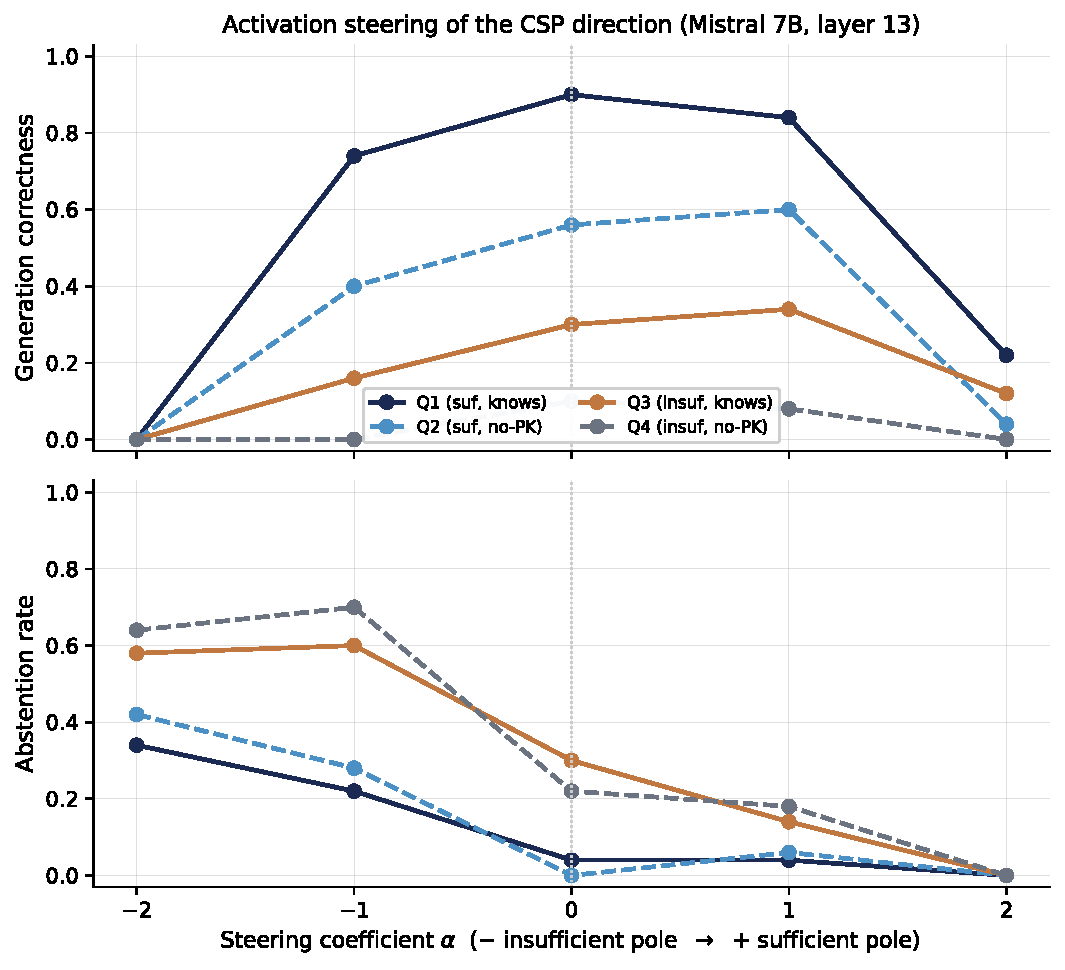
\includegraphics[width=0.8\textwidth]{Figure_E1.pdf}
\caption{Activation steering along the CSP probe direction in Mistral~7B (layer 13, injected across layers 11 to 15). Top: answer correctness. Bottom: abstention rate. Each point is 50 test items from one quadrant of the 2$\times$2 design. Negative coefficients push towards the insufficient pole and raise abstention, positive coefficients push towards the sufficient pole and suppress it, and $|\alpha| = 2$ collapses generation in both directions.}
\label{fig:steering}
\end{figure}

\section{Native Thinking Mode on Qwen3~8B}
\label{sec:thinking_app}
Qwen3~8B can generate an explicit reasoning trace before answering, which allows a test of whether deliberation closes the gap. We scored the test split in four ways: the raw prompt used for every other model, the same instruction inside the model's chat template with thinking disabled, the chat template with thinking enabled and a budget of 768 tokens (reading the confidence only after the closing think marker), and the chat template with thinking disabled but an explicit instruction to reason step by step before a final score line. Verbalized confidence reaches 0.729 AUROC on the raw prompt, 0.781 with the chat template, 0.771 with thinking enabled, and 0.802 with prompted chain-of-thought. With thinking enabled the model spends 299 reasoning tokens on average and exhausts the budget on 8.9\% of items. The native thinking mode therefore adds nothing over the same instruction without it, prompted reasoning adds 0.021, and all four variants remain 0.12 to 0.19 below the probe on the same model. On this evidence we do not expect native reasoning to close the gap, but the test covers one 8B model. The two frontier models were scored with their reasoning modes off, and the chain-of-thought result for Opus~4.7 in Table~\ref{tab:frontier} is prompted reasoning, not a native mode. A frontier model with its reasoning mode enabled remains to be evaluated.

\end{document}

